\PassOptionsToPackage{svgnames}{xcolor}
\documentclass[12pt]{article}



\usepackage[margin=1in]{geometry}  
\usepackage{graphicx}             
\usepackage{amsmath}              
\usepackage{amsfonts}              
\usepackage{framed}               
\usepackage{amssymb}
\usepackage{array}
\usepackage{amsthm}
\usepackage[nottoc]{tocbibind}
\usepackage{bm}

\usepackage{enumitem}
\usepackage{wrapfig}

  \newcommand\norm[1]{\left\lVert#1\right\rVert}
  \newcommand\TCP{\texttt{TCP} }
  \newcommand\UDP{\texttt{UDP} }
  \newcommand\IP{\texttt{IP} }
\setlength{\parindent}{0cm}
\setlength{\parskip}{0em}
\newcommand{\Lim}[1]{\raisebox{0.5ex}{\scalebox{0.8}{$\displaystyle \lim_{#1}\;$}}}
\newtheorem{definition}{Definition}[section]
\newtheorem{theorem}{Theorem}[section]
\newtheorem{notation}{Notation}[section]
\theoremstyle{definition}
\setcounter{tocdepth}{1}
\begin{document}

\title{Revision notes - CS2105}
\author{Ma Hongqiang}
\maketitle
\tableofcontents

\clearpage
%\twocolumn
\section{Introduction}
\subsection{What is the Internet?}
\begin{definition}[Internet]
\hfill\\\normalfont The \textit{Internet} is a network of connected computing devices known as \textbf{hosts} or \textbf{end systems}.\\
Hosts run \textbf{network applications}.
\end{definition}
Examples of hosts include PC, laptops, servers and smartphones.\\
Examples of network applications include Web, Pokemon Go, Skype.
\subsection{Network Edge}
Hosts access the Internet through access network. Hosts connect to the access network over different physical media.
\begin{itemize}
  \item \textbf{Guided media}: signals propagate in solid media, e.g. fiber
  \item \textbf{Unguided media}: signals propagate freely, e.g., Wi-Fi, cellular
\end{itemize}
\subsection{Network Core}
Network core consists of a mesh of interconnected routers. The data transmit through net via either \textbf{circuit switching} or \textbf{packet switching}.
\begin{definition}[Circuit Switching]
\hfill\\\normalfont In \textbf{circuit switching}, end-end resources allocated to and reserved for "call" between source and destination.
\begin{figure}[h]
\centering
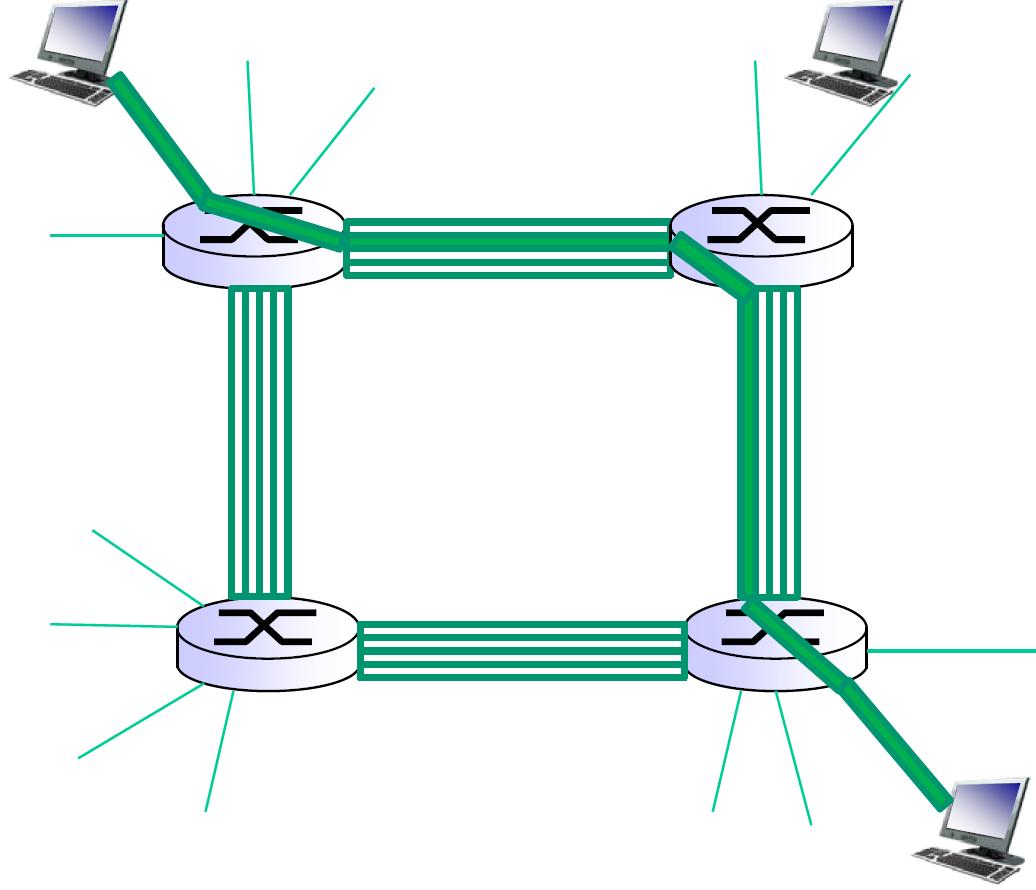
\includegraphics[width = 0.5\textwidth]{1_3_1.png}
\caption{In above diagram, each link has four circuits. A “call” gets 2nd circuit in top link and 1st circuit in right link.}
\end{figure}\\
Some properties of \textbf{circuit switching} include
\begin{itemize}
  \item call setup required
  \item circuit-like (guaranteed) performance
  \item circuit segment idle if not used by call (no sharing)
  \item \textit{commonly used in traditional telephone networks}
  \item divide link bandwidth into "pieces"
  \begin{itemize}
    \item frequency division
    \item time division
  \end{itemize}
\end{itemize}

\end{definition}
\begin{definition}[Packet Switching]
\hfill\\\normalfont In \textbf{packet switching}, host sending function by 
\begin{itemize}
\item breaking application message into smaller chunks known as \textbf{packets}, of length $L$ bits; and
\item transmitting packets onto the link at \textbf{trasmission rate}\footnote{link transmission rate is also known as \textbf{link capacity} or \textbf{link bandwidth}} $R$ bits/sec.
\end{itemize}
\end{definition}
\begin{definition}[Packet Trasmission Delay]
\hfill\\\normalfont Packet transmission delay, $d_{\text{trans}}$ is defined as time nedded to transmit $L$-bit packet onto link.
\[
d_{\text{trans}} = \frac{L}{R}
\]
\end{definition}
Packet switching adopts \textbf{store-and-forward} approach when a \textit{router} is encountered.
\begin{itemize}
  \item Packets are passed from one \textit{router} to the next, across links on path from source to destination.
  \item \textbf{Store and forward}: entire packet must arrive at a router before it can be transmitted on the next link.
\end{itemize}
\begin{figure}[h]
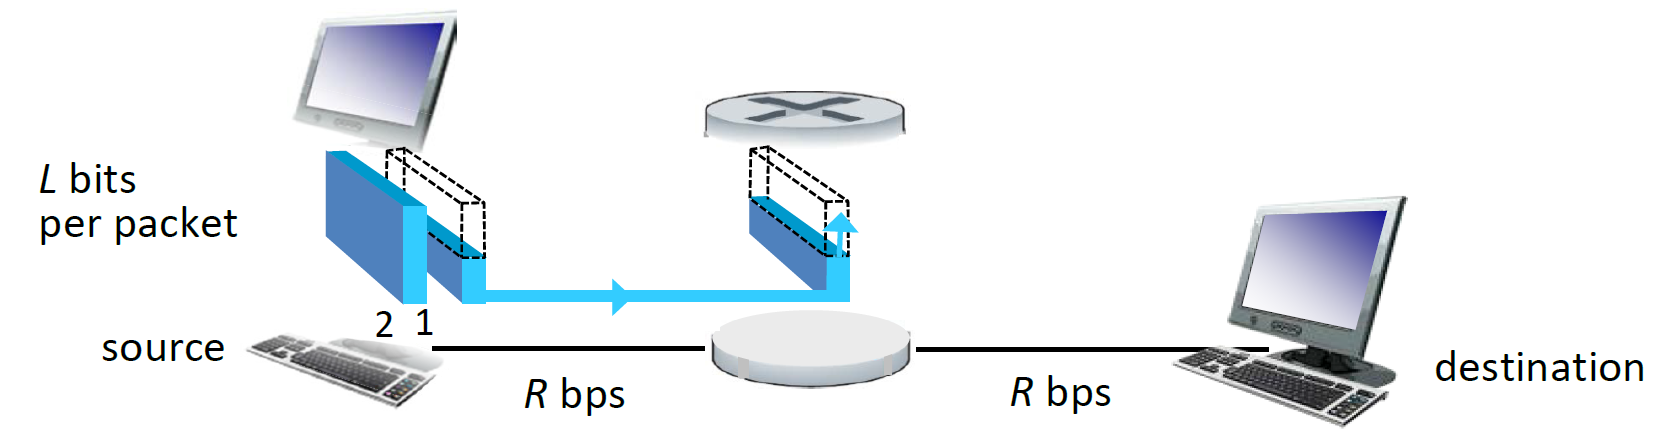
\includegraphics[width = \textwidth]{1_3_2.png}
\caption{End to end $d_{\text{trans}} = 2\times\frac{L}{R}$, assuming no other delays}
\end{figure}
\begin{definition}[Routing and Addressing]
\hfill\\\normalfont \textbf{Routers} determines source-destination route taken by packets by routing algorithms.\\
Addressing is achieved by each packet carrying source and destinaton information.
\end{definition}
Some properties of packet switching include
\begin{itemize}
  \item The Internet \textbf{is} a packet switching network.
  \item User A, B, $\ldots$'s packets \textit{share} network resources
  \item Resources are used on demand.
  \item Excessive congestion is possible.\footnote{These properties suggest bandwidth division into "pieces", dedicated allocation and resource reservation are not available.}
\end{itemize} 
\begin{definition}[Internet Structure: Network of Networks]
\hfill\\\normalfont
\vspace{-1em}
\begin{itemize}
  \item Hosts connect to Internet via access \textbf{ISPs}(Internet Service Providers)
  \item Access ISPs in turn must be interconnected.
  \item Resulting network of networks is very complex.\\Evolution was driven by \textit{economics} and \textit{national policies}.
  \item Therefore, the Internet is a "network-of-networks", organised into \underline{a}utonomous \underline{s}ystems(AS), each is owned by an organisation.
\end{itemize}
\end{definition}
\vspace{-1em}
\subsection{Delay, Loss and Throughput in Networks}
Recall, the algorithm of sneding a packet in a packet switching network is
\begin{enumerate}
  \item Sender transmit a packet onto the link as a sequence of bits.
  \item Bits are propagated to the next node(e.g. a router) on the link.
  \item Router stores, processes and forwards the packet to the next link.
  \item Steps 2 and 3 repeat till the packet arrives at the receiver.
\end{enumerate}
Delay and Loss could occur as packets need to queue in router buffers, waiting for turn to be send out one by one.
\begin{figure}[h]
\centering
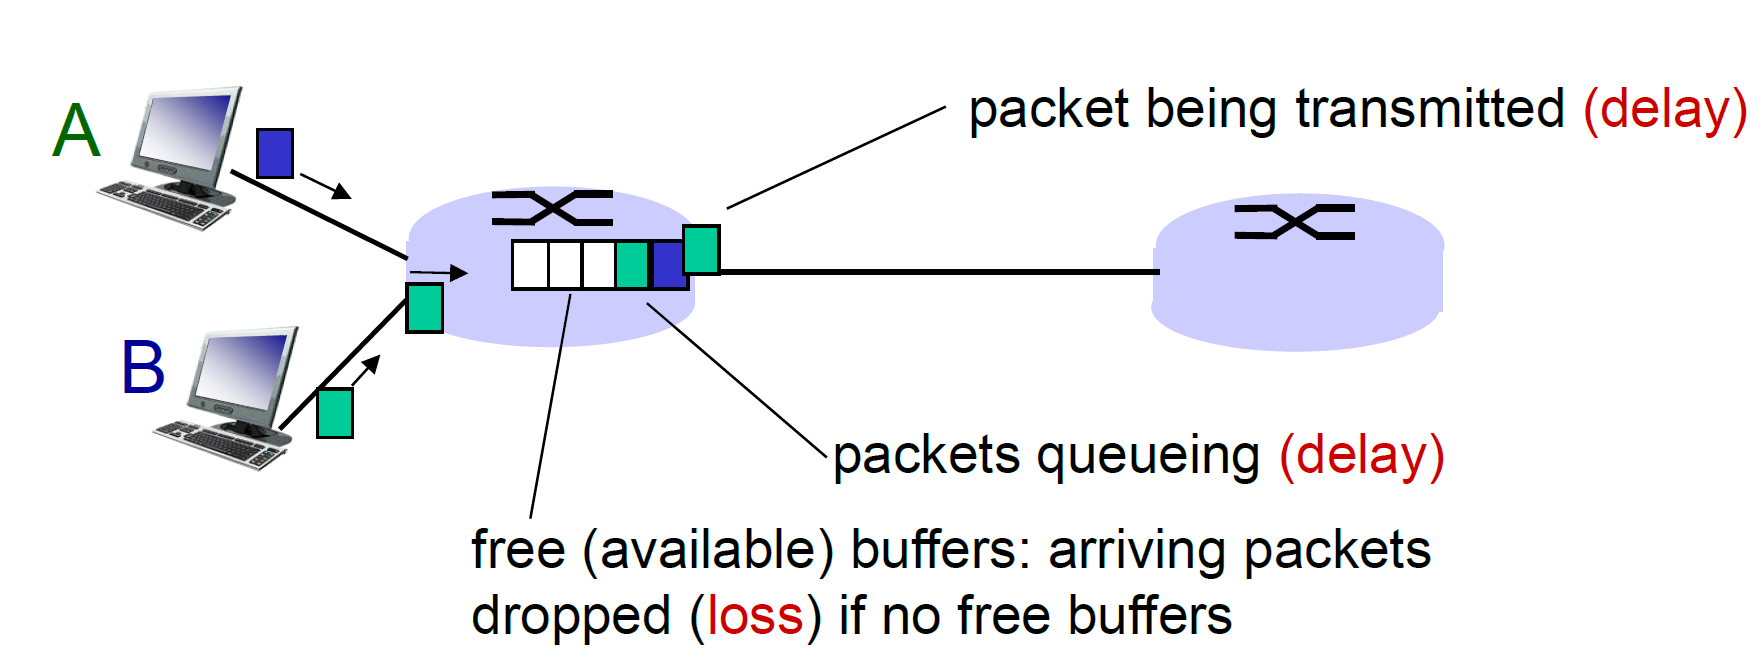
\includegraphics[width = 0.5\textwidth]{1_4_1.png}
\end{figure}\\
\begin{itemize}
  \item Queue(aka \textbf{buffer}) of a router has finite capacity.
  \item Packet arriving to full queue will be dropped(aka lost).
  \item Lost packet may be retransmitted by previous node, by source host, or not at all.
\end{itemize}
\begin{definition}[Four Sources of End-to-end Packet Delay]
\hfill\\\normalfont 
End-to-end packet delay is the time taken for a packet to travel from source to destination. It consists of:
\begin{itemize}
  \item transmission delay
  \item propagation delay
  \item processing delay
  \item queueing delay
\end{itemize}
\begin{table}[h]
\hspace{-4em}
\begin{tabular}{|p{5.5cm}|p{4cm}|p{4.5cm}|p{4.5cm}|}
\hline
$d_\text{proc}$: nodal processing delay&$d_\text{queue}$: queueing delay&$d_\text{trans}$: transmission delay&$d_\text{prop}$: propagation delay\\\hline
\begin{itemize}[leftmargin=3mm]
  \item check bit errors
  \item determine output link
  \item typically $<$ msec
\end{itemize}&
\begin{itemize}[leftmargin=3mm]
  \item time waiting in the queue for transmission
  \item dependes on congestion level of router
\end{itemize}&
\begin{itemize}[leftmargin=3mm]
  \item $L$: packet length
  \item $R$: link bandwidth
  \item $d_\text{trans} = \frac{L}{R}$
\end{itemize}&
\begin{itemize}[leftmargin=3mm]
  \item $d$: length of physical link
  \item $s$: propagation speed in medium\newline($\sim 2\times 10^8$m/sec)
  \item $d_\text{prop} = \frac{d}{s}$
\end{itemize}
\\\hline
\end{tabular}
\end{table}
\end{definition}
\begin{definition}[Throughput]
\hfill\\\normalfont \textbf{Throughput} is defined as how many bits can be transmitted per unit time.\\
\end{definition}
\begin{figure}[h]
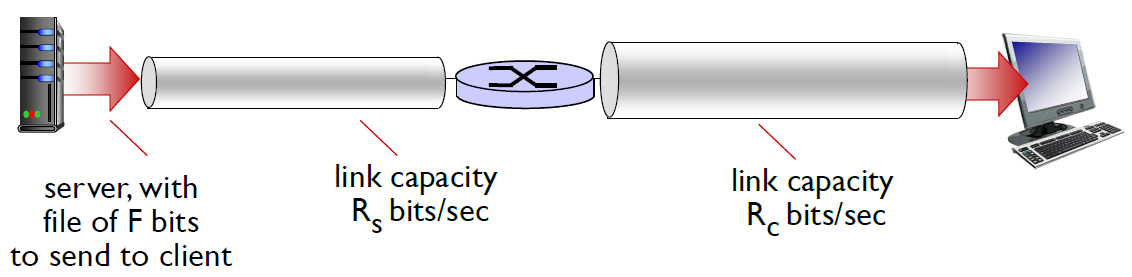
\includegraphics[width = \textwidth]{1_4_2.png}
\caption{The throughput is $\frac{F}{\left(\frac{F}{R_s}+\frac{F}{R_c}\right)}=\frac{R_sR_c}{R_s+R_c}$}
\end{figure}
\clearpage
The difference between throughput and link capacity is that
\begin{itemize}
  \item Throughput is measured for end-to-end communication.
  \item Link capacity(bandwidth) is meant for a specific link.
\end{itemize}
\subsection{Protocol Layers and Service Models}
The Internet supports various network applications. Network applications exchange messages and communicate among peers according to \textbf{protocols}.
\begin{definition}[Protocol]
\hfill\\\normalfont \textbf{Protocols} define \textit{format} and \textit{order} of messages exchanged and the \textit{actions} taken after messages are sent or received.
\end{definition}
Protocols in the Internet are logically organised into "layers" according to their purposes.
\begin{itemize}
  \item Each layer provides a service.
  \item Simple interfaces between layers
  \item Hide details from each other
\end{itemize}
\begin{definition}[Internet Protocol Stack]
\hfill\\\normalfont The Internet consists of five layers.
\begin{itemize}
  \item \textbf{Application}: supporting network applications, e.g. FTP, SMTP, HTTP
  \item \textbf{Transport}: process-to-process data transfer, e.g. TCP, UDP
  \item \textbf{Network}: routing of datagrams from source to destination, e.g. IP
  \item \textbf{Link}: data transfer between neighbouring network elements,e.g. Ethernet, 802.11
  \item \textbf{Physical}: bits "on the wire"
\end{itemize}
\end{definition}
\clearpage
\section{Application Layer}
\subsection{Principle of Network Applications}
\textbf{Application architectures} refer to possible structures of network applications, which include:
\begin{itemize}
  \item Client-server
  \item Peer-to-peer(P2P)
  \item Hybrid of client-server and P2P
\end{itemize}
\begin{definition}[Client-Server Architecture]
\hfill\\\normalfont In \textbf{client-server} architecture,\\
\textbf{Server}:
\begin{itemize}
  \item Waits for incoming requests
  \item Provides requested service to client
\end{itemize}
\text{Client}:
\begin{itemize}
  \item Initiates contact with server("speak first")
  \item Typically requests service from server
  \item For Web, client is usually implemented in browser
\end{itemize}
\end{definition}
\begin{definition}[P2P Architecture]
\hfill\\\normalfont In \textbf{P2P} Architecture,
\begin{itemize}
\item \textit{No} always-on server
\item Arbitrary end systems directly communicate.
\item Peers request service from other peers, provide service in return to other peers.
\end{itemize}
P2P Architecture is highly scalable but difficult to manage.
\end{definition}
An example of Hybrid of Client-Server and P2P architecture is the instant messaging, where
\begin{itemize}
  \item Chatting between two users is \textbf{P2P}
  \item Presence detection/location is \textbf{centralised}
\end{itemize}
Usually for applications, some considerations of \textit{transport} service include
\begin{itemize}
  \item Data integrity
  \item Throughput
  \item Timing
  \item Security
\end{itemize}
\begin{definition}[Two Internet Transport Protocols]
\hfill\\\normalfont Two Internet Transport Protocols are \texttt{TCP} and \texttt{UDP}. The main difference is that \texttt{TCP} is reliable while \texttt{UDP} is not. In detail, \\
\texttt{TCP} service offers:
\begin{itemize}
  \item \textbf{reliable transport} between sending and receiving pocess
  \item \textbf{flow control}: sender won't overwhelm receiver
  \item \textbf{congestion control}: throttle sender when network is overloaded
\end{itemize}
However, \texttt{TCP} does \textit{not} provide: timing, minimum throughput guarantee, security.\\
In contrast, \texttt{UDP} service provide \textbf{unreliable} data transfer between sending and receiving process. It does \textit{not} provide: reliability, flow control, congestion control, timing, throughput guarantee or security.
\end{definition}
For \textbf{application layer protocol} which is over transport layer protocol, instead it defines
\begin{itemize}
  \item Types of messages exchanged: e.g., request, response
  \item Message syntax: what field in messages and how fields are delineated
  \item Message semantics: meaning of information in fields
  \item Rules: for when and how applications send and respond to messages
  \item Open protocols: defined in RFCs; allow for interoperability; e.g., \texttt{HTTP}, \texttt{SMTP}
  \item Proprietary protocols, e.g., Skype
\end{itemize}
\subsection{Web and \texttt{HTTP}}
\begin{definition}[Web Page]
\hfill\\\normalfont A \textbf{Web page} typically consists of:
\begin{itemize}
  \item base \texttt{HTML} file, and
  \item several referenced \textit{objects}\\An object can be HTML file, JPEG image etc.\\Each object is addressable by a \textbf{URL},e.g.,
  \[
\underbrace{\texttt{www.comp.nus.edu.sg}}_{\text{host name}}\underbrace{\texttt{/~cs2105/img/doge.jpg}}_{\text{path name}}
  \]

\end{itemize}
\end{definition}
\begin{definition}[\texttt{HTTP}]
\hfill\\\normalfont \texttt{HTTP} refers to \textbf{\underline{H}yper\underline{t}ext \underline{t}ransfer \underline{p}rotocol}.\\\texttt{HTTP}
\begin{itemize}
  \item is Web's application layer protocol
  \item usees client/server model
  \begin{itemize}
    \item \textbf{client}: usually is browser that requests, receives and displays Web objects
    \item \textbf{server}: Web server sends objects in response to requests
  \end{itemize}
\end{itemize}
\end{definition} 
Note that \texttt{HTTP} uses \texttt{TCP} as transport service.\\
\subsubsection{Non-persistent \texttt{HTTP}}
In \textbf{non-persistent} \texttt{HTTP/1.0},
\begin{enumerate}
  \item Client initiates \texttt{TCP} connection to server.
  \item Server accepts \texttt{TCP} connection request from client.
  \item \texttt{HTTP} messages are exchanged between browser(\texttt{HTTP} client) and Web server(\texttt{HTTP} server) over \texttt{TCP} connection.
  \item \texttt{TCP} connection closed.
  \item \texttt{HTTP} client receives response message containing HTML file, displays HTML. Parsing HTML file, client notices referenced objects.
  \item Step 1$\sim$5 repeated for the referenced objects. 
\end{enumerate}
\begin{definition}[Round Trip Time(RTT)]
\hfill\\\normalfont \textbf{Round trip time}(RTT) refers to the time for a packet to travel from client to server and go back.
\end{definition}
\begin{minipage}{0.45\textwidth}
Clearly, the \texttt{HTTP} \textbf{response time} for one object transfer equals the sum of:
\begin{itemize}
  \item one RTT to establish \texttt{TCP} connection
  \item one RTT for \texttt{HTTP} request and the first few bytes of \texttt{HTTP} response to return
  \item file transimission time
\end{itemize}
As a result, the \textbf{non-persistent} \texttt{HTTP} response time = \[2\times \text{RTT}+\text{file trasmission time}\].

\end{minipage}
\hfill
\begin{minipage}{0.5\textwidth}
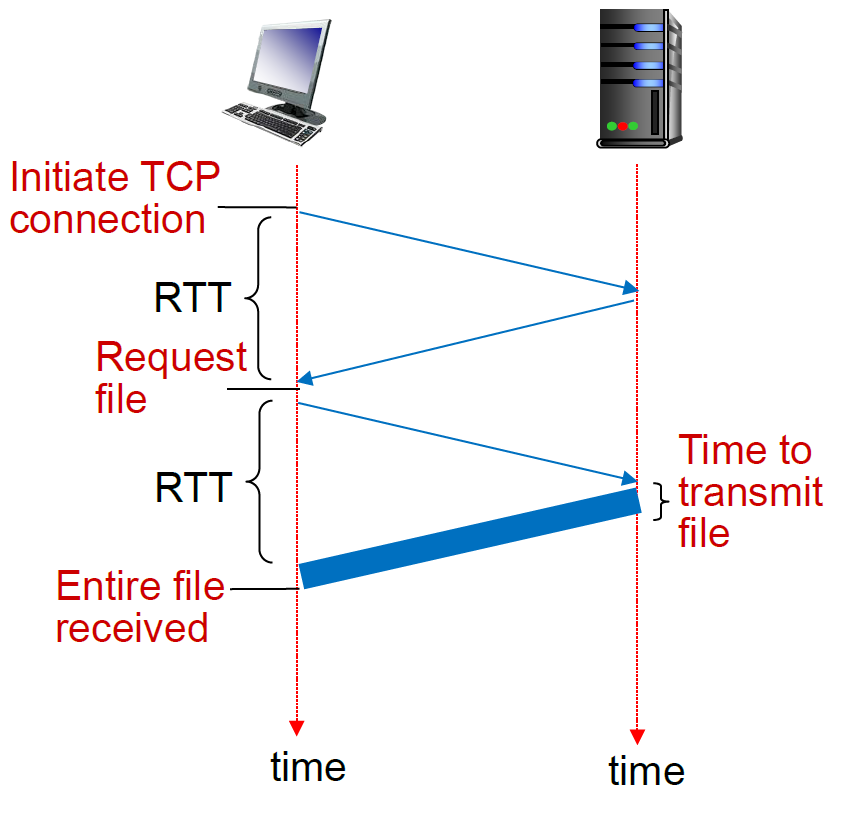
\includegraphics[width = 8cm]{2_2_1.png}
\end{minipage}
\subsubsection{Persistent \texttt{HTTP}}
The problems of non-persistent \texttt{HTTP} include:
\begin{itemize}
  \item requires 2 RTTs per object
  \item OS overhead for \textit{each} \texttt{TCP} connection
  \item browsers often open parallel \texttt{TCP} connections to fetch referenced objects
\end{itemize}
\textbf{Persistent} \texttt{HTTP/1.1} solves these issues by:
\begin{itemize}
  \item server leaves connection open after sending response
  \item subsequent \texttt{HTTP} messages between same client/server sent over the same \texttt{TCP} connection
  \item client sends requests as soon as it encounters a referenced object(\textit{persistent with pipelining})
  \item as little as one RTT for all the referenced objects
\end{itemize}
Example \texttt{HTTP} request message usually entails both \textbf{request} and \textbf{response}.\\
A \texttt{HTTP} \textbf{request} message looks like:

\begin{verbatim}
GET /~cs2105/demo.html HTTP/1.1
Host: www.comp.nus.edu.sg
User-Agent: Mozilla/5.0
Connection: close
\r\n
\end{verbatim}
The 1st line is the request line. Subsequent 3 lines are header lines. Last extra blank line indicates end of header lines.\\
A \texttt{HTTP} \textbf{response} message looks like:
\begin{verbatim}
HTTP/1.1 200 OK
Date: Thu, 15 Jan 2015 13:02:41 GMT
Server: Apache/2.4.6 (Unix)
Content-Type: text/html
\r\n
data data data data ...
\end{verbatim}
The 1st line is the protocol status line. Subsequent 3 lines are header lines. After the extra blank line is the data of the requested HTML file.
\subsubsection{Cookies}
\texttt{HTTP} is desisned to be \textbf{stateless}, in a sense that server maintains \textit{no} information about past client requests.\\
However, sometimes it is good to maintain states(history) at server/client over multiple transactions.
\begin{definition}[Cookies]
\hfill\\\normalfont Cookies allow sites to keep track of users.\\Cookie technology has four components:
\begin{itemize}
  \item A cookie header line in the \texttt{HTTP} response message
  \item A cookie header line in the \texttt{HTTP} request message
  \item A cookie file kept on the user's end system and managed by the user's browser
  \item A back-end database at the Web site
\end{itemize}
\begin{figure}[h]
\centering
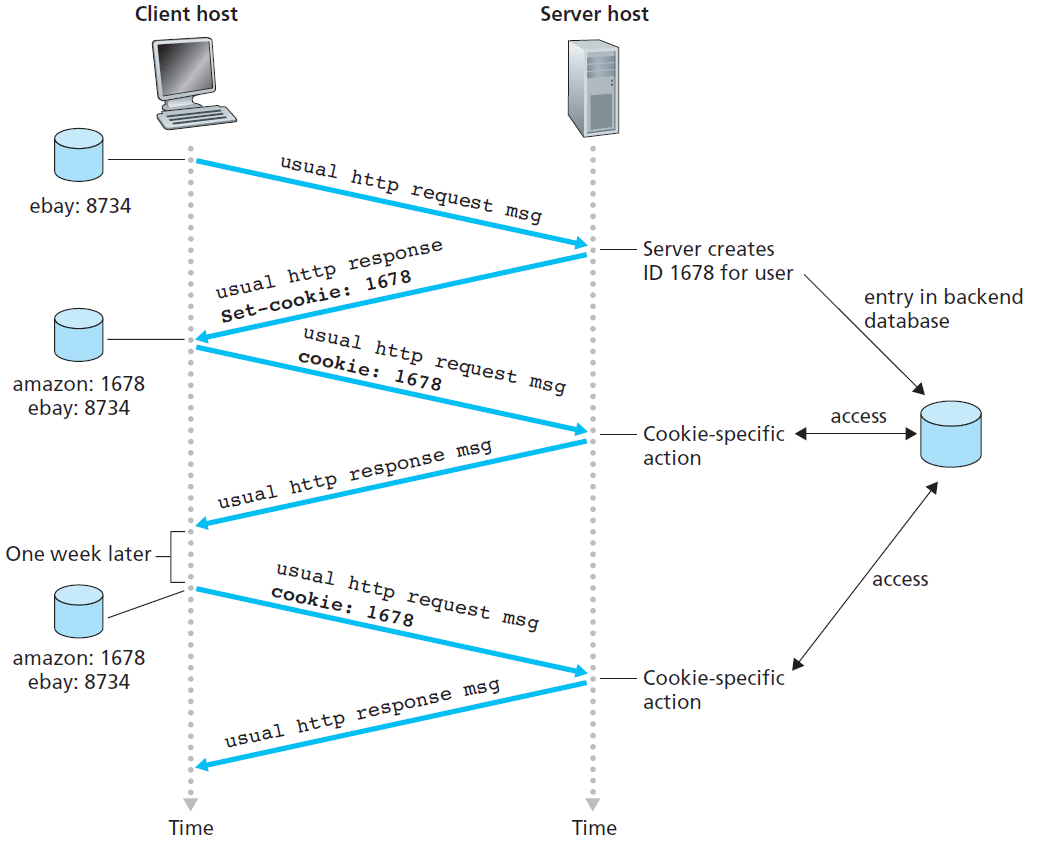
\includegraphics[width = 0.8\textwidth]{2_2_2.png}
\end{figure}
\end{definition}
\subsubsection{Conditional \texttt{GET}}
The goal of conditional \texttt{GET} is to \textbf{not} send object if client cache has \textbf{up-to-date} cached version.\\
In the client cache, date of cached copy in \texttt{HTTP} request is specified by \texttt{If-modified-since: <date>}.\\
In the server response, no object will be contained in the response if cached copy is up-to-date, and return \texttt{HTTP/1.0 304 Not Modified}.
\subsection{Domain Name System}
There are two ways to identify a host:
\begin{enumerate}
  \item \textbf{Hostname}, e.g., www.comp.nus.edu.sg
  \item \texttt{IP} \textbf{address}, e.g., 137.132.80.57
\end{enumerate}
\begin{definition}[DNS]
\hfill\\\normalfont Domain Name System(DNS) translates between hostname and \texttt{IP} address.
\end{definition}
A client must carry out a DNS query to determine the \texttt{IP} address corresponding to the server name (e.g., www.comp.nus.edu.sg) prior to the connection.
\begin{definition}[DNS Resource Records]
\hfill\\\normalfont \textbf{DNS resource records} are mappings between host names and \texttt{IP} addresses and others.
The format of resource records is
\begin{center}
\fbox{\begin{minipage}{0.4\textwidth}\centering\texttt{(name, value, type, TTL)}\end{minipage}}
\end{center}
There are 4 \texttt{type} if resource records.
\begin{enumerate}
  \item \texttt{type} = A: \texttt{(hostname, IP address, A, TTL)}
  \item \texttt{type} = CNAME: \texttt{(caconical name, real name, CNAME, TTL)}
  \item \texttt{type} = NS: \texttt{(domain name, hostname of authoritative name server for this domain, NS, TTL)}
  \item \texttt{type} = MX: \texttt{(domain name, mail server, MX, TTL)}
\end{enumerate}
\end{definition}
DNS stores resource records in distributed databases implemented in hierarchy of many name servers.
\begin{figure}[h]
\centering
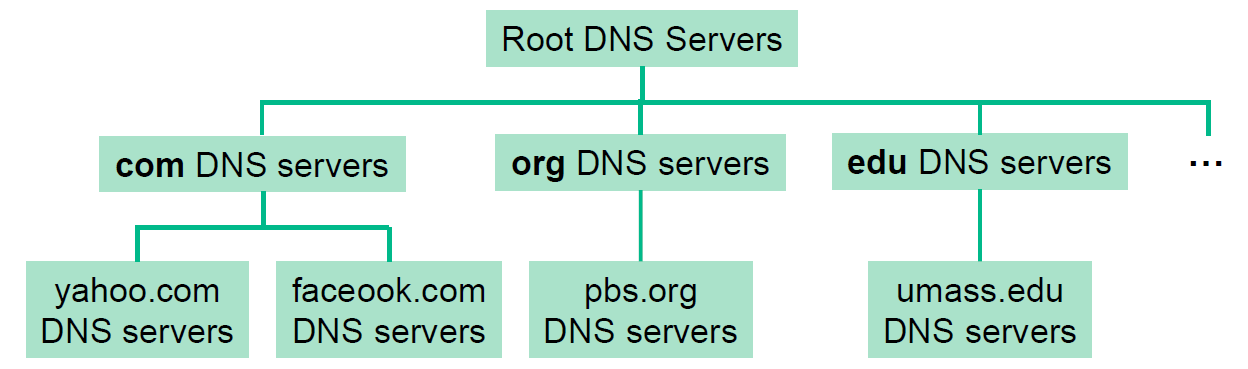
\includegraphics[width = 0.7\textwidth]{2_2_3.png}
\end{figure}
For example, if a client wants \texttt{IP} address for www.facebook.com:
\begin{itemize}
  \item Client queries root server to find .com DNS server

  \item Client queries .com DNS server to get facebook.com DNS server

  \item Client queries facebook.com DNS server to get \texttt{IP} address for www.facebook.com
\end{itemize}
Here, \textbf{root servers} answer requests for records in the root zone by returning a list of the authoritative name servers for the appropriate top-level domain(TLD).\\
\textbf{Top level domain}(TLD) servers us responsible for com,org,net.edu and all top-level country domains and returns a list of authoritative servers.\\
\textbf{Authoritative servers} are organisation's own DNS servers, providing authoritative hostname to \texttt{IP} mappings for organisation's named hosts(e.g., web, mail). They can be maintained by organisation or service provider.\\
\textbf{Local DNS server} is also called \textit{default name server}. It does not strictly belong to the hierarchy; each ISP has one local DNS server. When host makes a DNS query, query is sent to its local DNS server and
\begin{itemize}
  \item Retrieve name-to-address translation from local cache;
  \item if answer is not found \textit{locally}, acts as proxy and forwards query into hierarchy if answer is not found locally
  \item Once it learns mapping, it caches mapping. Cache entries will expire after Time to Live(TTL) countdown.
\end{itemize}
Note that DNS runs over \texttt{UDP} for speed. \texttt{UDP} is faster since compared to \texttt{TCP}, it avoids one RTT induced by \texttt{TCP} handshake.
\clearpage
\section{Socket Programming}
\subsection{Processes}
\begin{definition}[Process]
\hfill\\\normalfont Applications runs in hosts as \textbf{processes}.
\begin{itemize}
  \item Within the \textit{same} host, two processes communicate using \textbf{inter-process communication} (defined by OS).
  \item Processes in \textit{different} hosts communicate by exchanging \textbf{messages} (according to protocols).
\end{itemize}
\end{definition}
In Client/Server model, \textbf{server process} waits to be contacted; \textbf{client process} initiates the communication.
\begin{theorem}[Addressing processes]
\hfill\\\normalfont A process is identified by (\textbf{IP address}, \textbf{port number}), where \textbf{port number} is a 16-bit integer.
\end{theorem}
\clearpage
\subsection{Sockets}
\begin{definition}[Socket]
\hfill\\\normalfont \textbf{Socket} is the software interface between app processes and transport layer protocols.
\begin{itemize}
  \item Process sends/receives messages to/from its socket.
  \item Programming-wise: a set of \textbf{API} calls
\end{itemize}
\end{definition}
Refer to Lecture Notes for programming details.
\clearpage
\section{Transport Layer Protocol}
\subsection{Transport-layer Services}
Internet transport layer protocols mainly are:
\begin{itemize}
  \item \TCP: connection-oriented and reliable
  \item \UDP: connection-less and unreliable
\end{itemize}
Transport layer protocols run in hosts.
\begin{itemize}
  \item Sender side:
  \begin{itemize}
    \item breaks app message into \textbf{segments}
    \item passes them to network layer
  \end{itemize}
  \item Receiver side:
  \begin{itemize}
    \item reassembles segments into message
    \item passes it to application layer
  \end{itemize}
\end{itemize}
\subsection{\UDP: User Datagram Protocol}
\UDP adds very little service on top of $\texttt{IP}$:
\begin{itemize}
  \item Connectionless multiplexing/de-multiplexing
  \item Checksum
\end{itemize}
\UDP transmission is \textbf{unreliable}. Therefore, to achieve reliable transmission over \UDP, application layer protocol should implement error detection and recovery mechanism.\\
\UDP has advantage over \TCP in
\begin{itemize}
  \item No connection establishment (No handshake delay)
  \item Simple: no connection state at sender and receiver
  \item Small header size
  \item No congestion control
\end{itemize}
\subsubsection{Connectionless De-multiplexing}
Connectionless de-multiplexing is achieved by information on port numbers.
\begin{itemize}
  \item \UDP sender:
  \begin{itemize}
    \item creates a socket with \textbf{local port number}.
    \item When creating a datagram to send to \UDP socket, sender must specify \textbf{destination }\texttt{IP}\textbf{ address} and \textbf{port number}.
  \end{itemize}
  \item When \UDP receiver receives a \UDP segment:
  \begin{itemize}
    \item Checks \textbf{destination port number} in segment.
    \item Directs \UDP segment to the socket with that port number.
    \item \texttt{IP} datagram from different sources with the \textbf{same destination port number} will be directed to the same \UDP socket at destination.
  \end{itemize}
\end{itemize}
\begin{figure}[h]
\centering
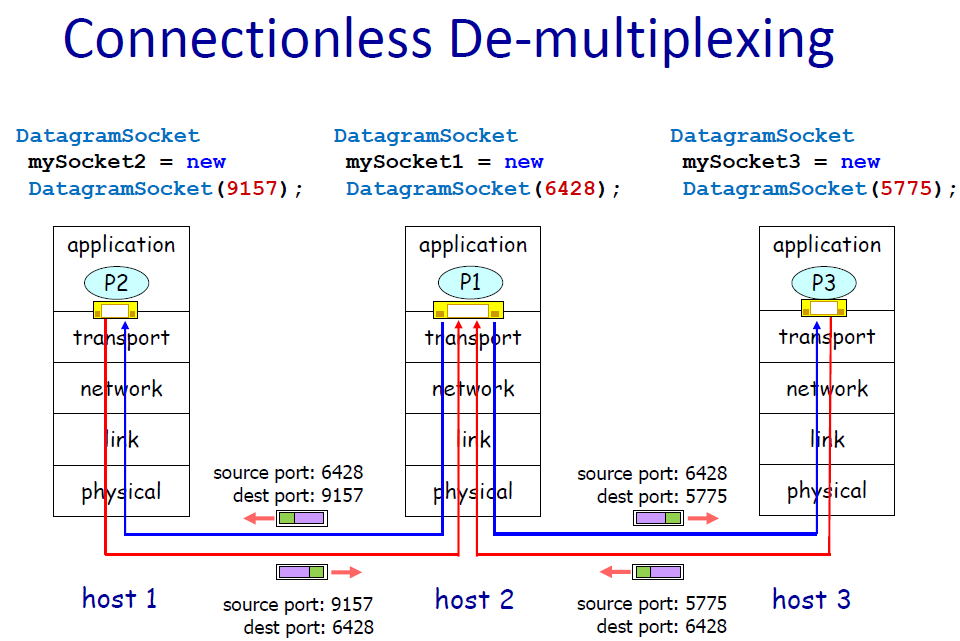
\includegraphics[width = 0.7\textwidth]{4_2_1.png}
\end{figure}
\subsubsection{\UDP Header}
\begin{definition}[\UDP Header]
\hfill\\\normalfont \UDP \textbf{header} consists of 64 bits:
\begin{figure}[h]
\begin{minipage}{0.55\textwidth}
\begin{itemize}
  \item bit $1\sim16$: source port number ($0\sim65535$)
  \item bit $17\sim32$: destination port number ($0\sim65535$)
  \item bit $33\sim48$: length of \UDP segment in \textbf{bytes}, including header
  \item bit $49\sim64$: checksum
\end{itemize}
\end{minipage}\hfill\begin{minipage}{0.3\textwidth}
\centering
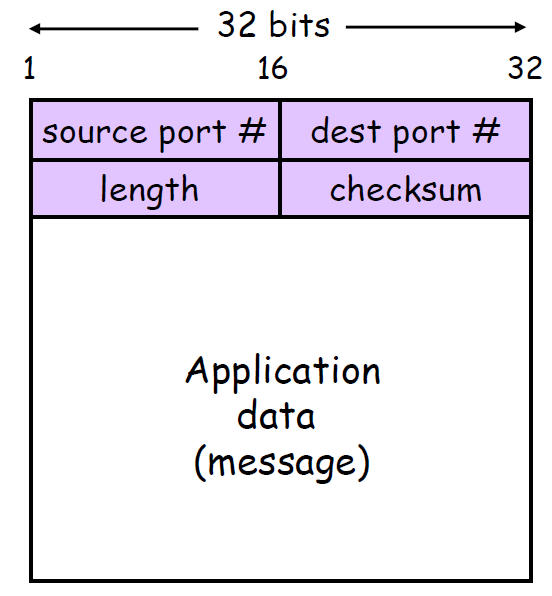
\includegraphics[width=\textwidth]{4_2_2.png}
\end{minipage}
\end{figure}
\end{definition}
\clearpage
\subsubsection{\UDP Checksum}
\UDP Checksum is used to detect errors in transmitted segment.\\
\begin{itemize}
  \item Sender
  \begin{enumerate}
    \item Compute checksum value
    \item Put checksum value into \UDP checksum field
  \end{enumerate}
  \item Receiver
  \begin{enumerate}
    \item Computer checksum of received segment
    \item Check if computed checksum equals checksum field value
    \begin{itemize}
      \item NO -- error detected
      \item YES -- no error with respect to the checksum check
    \end{itemize}
  \end{enumerate}
\end{itemize}
\begin{theorem}[Checksum Computation]
\hfill\\\normalfont CHecksum is computed accordingly
\begin{enumerate}
  \item Treat \UDP segment as a sequence of \textbf{16-bit} integers.
  \item Apply binary addition on every 16-bit integer. If the last integer is of length less than 16 bit, add zeroes to the right of last integer until 16 bit is reached.
  \item Carry (if any) from the most significant bit will be added to the result
  \item Compute 1's complement to get \UDP checksum.
\end{enumerate}
\end{theorem}
\subsection{Principle of Reliable Data Transfer 3.0}
In this section, we assume the underlying channel
\begin{itemize}
  \item \textit{may} flip bits in packets
  \item \textit{may} lose packets
  \item \textit{may} incur arbitrarily long packet delay
  \item \textit{will NOT} reorder packets
\end{itemize}
Reliable data transfer involves a sender and a receiver.
\begin{itemize}
\item The sender sends out \textbf{segments};
\item the receiver replies \textbf{ACK} message.
\end{itemize}
A \textbf{sequence ID} is assigned by sender to each packet. \textbf{Acknowledgements} contains the sequence ID of the last successfully received packet.\\ 
\subsubsection{Behavior of Sender}
In reliable data transfer, sender maintains a \textbf{timer}. The timer will start when a segment is sent and stops by receiving ACK with sequence ID of this segment. Until then, another packet with a different sequence ID will be sent, with the whole process again. Otherwise, the timer will timeout, in which case this same packet is sent again.\\All incoming packets(ACK) will be ignored if the sender waits to send, in which case there is no timer running.
\subsubsection{Behaviour of the receiver}
The data transfer is initiated by sender sending the first segment. On receiving a packet, \textit{corrupted} copy will trigger an ACK of last correctly received copy. Receiver will also check the sequence ID for duplicate segment for duplicated copy. However, ACK of that copy's sequence ID will be sent regardless of whether it is a duplicate or not; the only difference is that duplicated copy will be discarded. If it is not corrupted and not a duplicate packet, it will be delivered to application layer.
\subsubsection{Bit Error}
Bit error occurs when some bits of the segment are flipped.\\
Bit error can occur in
\begin{itemize}
  \item \textbf{segment}, in which case
  \begin{enumerate}
    \item receiver detects bit error using checksum
    \item receiver ignores packet
    \item receives send ACK with sequence ID of last successfully transmitted segment
  \end{enumerate}
  \item ACK message, in which case
  \begin{enumerate}
    \item sender will ignore the corrupted ACK
  \end{enumerate}
\end{itemize}
\subsubsection{Packet Loss}
Packet loss occurs in
\begin{itemize}
  \item Segment, in which case receiver will do nothing;
  \item ACK message, in which case sender will do nothing.
\end{itemize}
\subsubsection{Arbitrarily Long Packet Delay}
Arbitrarily long packet delay can occur in
\begin{itemize}
  \item Segment, in which case receiver reply ACK accordingly once received;
  \item ACK message, in which case sender will only act according to timer.
\end{itemize}
\subsubsection{Finite State Machine Diagram of Reliable Transfer Protocol}
\begin{figure}[h]
\centering
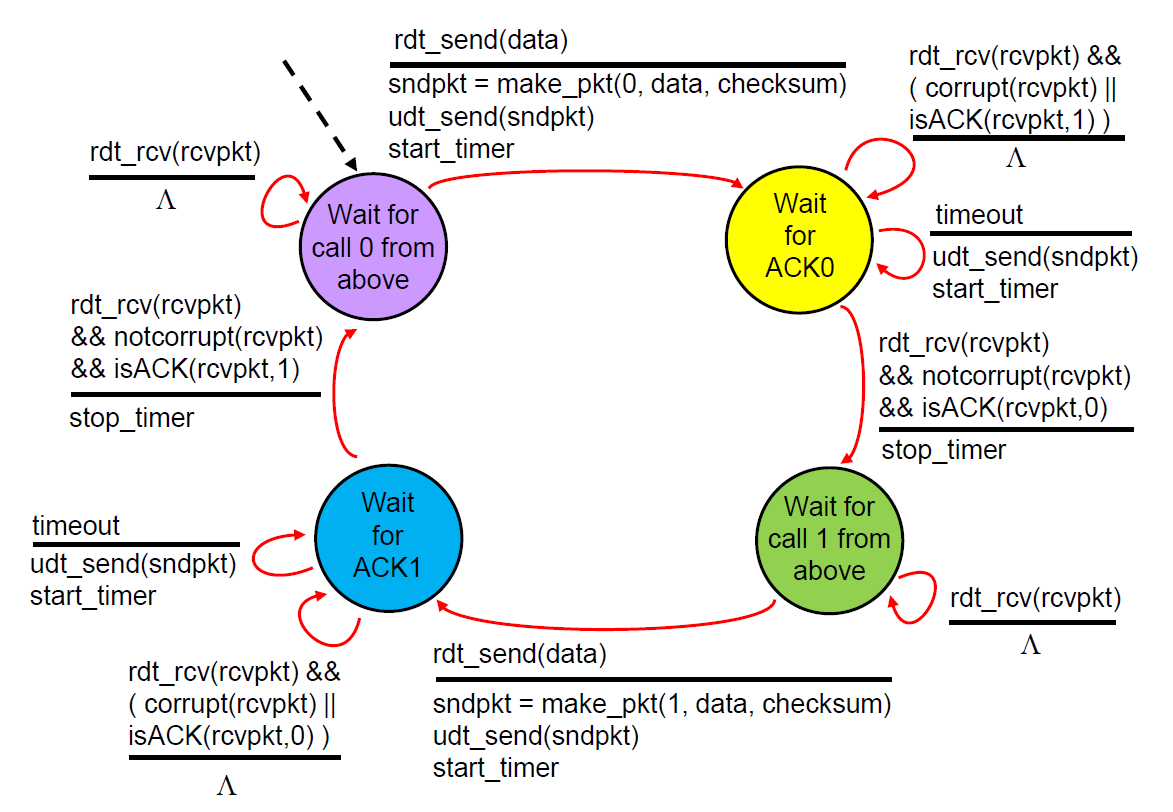
\includegraphics[width = 0.9\textwidth]{4_3_1.png}
\caption{Reliable Data Transfer Sender Finite State Machine}
\end{figure}
\begin{figure}[h]
\centering
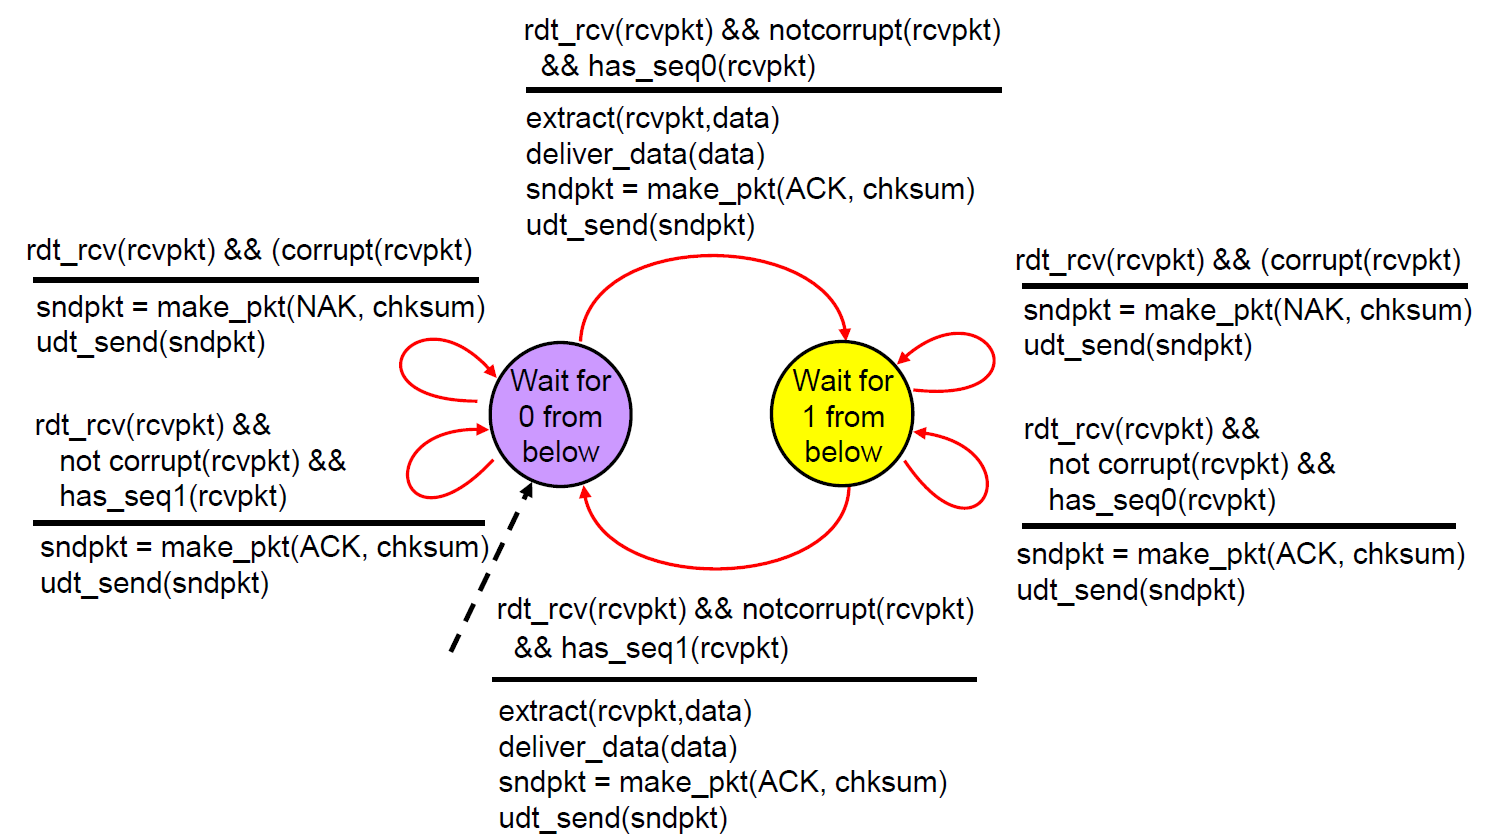
\includegraphics[width = 0.9\textwidth]{4_3_2.png}
\caption{Reliable Data Transfer Receiver Finite State Machine}
\end{figure}
\clearpage
\subsubsection{Performance of rdt 3.0}
\begin{definition}[Utilisation]
\hfill\\\normalfont \textbf{Utilisation} is defined as the fraction of time sender is busy sending.
\end{definition}
rdt 3.0 stinks in performance, given its \textbf{stop-and-wait} nature. \textbf{Pipelining} can be used to increase utilisation, which allows multiple "in-flight", yet-to-be-acknowledged packets.\\Two generic form of pipelined protocols are
\begin{itemize}
\item Go-Back-N
\item Selective Repeat
\end{itemize}
\subsection{Go-back-N}
\subsubsection{Sender Behaviour}
\begin{itemize}
\item Sender maintains a window size of $N$, i.e., there can be $N$ packets in pipeline, where the \textit{first} is unACKed.
\item There will be a timer for the first packet in the window.
\item Packets in the window will be \textit{cumulatively} ACKed.
\item If the sender receive ACK of a packet with sequence ID $k$, all packet no later than sequence ID $k$ will be ACKed; the window will slide until the next packet of sequence ID $k+1$.\footnote{This is due to cumulative acknowledgement.} Sender will send the packets newly entered in the window. If there is no timer running, start the timer to take the oldest unACKed packet. 
\item Else, the first packet's timer will timeout by receiving no ACK with sequence ID in the window. The sender will retransmit all the packets in the window.
\end{itemize}
\subsubsection{Receiver Behaviour}
\begin{itemize}
  \item Same as rdt 3.0, corrupted packets will be discarded. 
  \item Acknowledge packet in order, by maintaining an \texttt{expectedSeqNum}. Any packet of different sequence ID from \texttt{expectedSeqNum} will be discarded.
  \item In all cases, acknowledgement is \textbf{cumulative}. \\When the expected packet is received, ACK with sequence ID \texttt{expectedSeqNum} will be sent and \texttt{expectedSeqNum++}.\\When other packet is received, ACK with sequence ID \texttt{expectedSeqNum-1} will be sent.\\
  As such, ACK $k$ means all packets up to $k$ are received.
  \end{itemize}
The benefit of cumulative ACK is that lost ACK packet will not cause retransmission as long as one ACK packet after this lost packet is received by sender before timeout. Therefore, timeout value shall be delicately chosen.\\

However, Go-back-N will waste network resources in a sense corrupt-free packet will be discarded merely for being out-of-order. 
\subsection{Selective Repeat}
Selective repeat solves the problem by \textbf{buffering} the out-of-order packets.
\subsubsection{Sender Behaviour}
\begin{itemize}
\item Sender maintains a window size of $N$. Window will be maintained such that the first packet of the window is unACKed.
\item There will be a timer for \textit{every} packet in the window.
\item Packets in the window will be \textit{individually} ACKed.
\item If one timer timeout, \textit{only} the timed-out packet will be resent.
\item Upon sliding of window due to acknowledgement of first packet, packets newly entered the window will be sent.
\end{itemize}
\subsubsection{Receiver Behaviour}
\begin{itemize}
  \item Same as rdt 3.0, corrupted packets will be discarded.
  \item Acknowledge packet individually.
  \item Maintain a \textbf{receiver window} of equal length $N$ to the sender window. The first packet in receiver window is not received.
  \item All the packets received \textit{correctly}, which either are inside the receiver window, or outside the receiver window but within just one window length $N$ before the first UnACKed packet, will fire an individual ACK message.
  \item If packets correctly received is in-order, all consecutive packets buffered in the receiver window will be delivered to application layer. The receiver window will slide to maintain the "first UnACKed" property.
  \item If packets correctly received is out-of-order, it will be buffered.
  \item All the packets \textit{corrupted}, or out of the specified range before will not be buffered, and will not fire ACK.
  \end{itemize}
  \clearpage
\section{\TCP: Transport Control Protocol}
\TCP is \textbf{connection-oriented} in a sense handshaking is required before sending application data. \\\TCP supports a \textbf{reliable, in-order} byte stream: Application passes data to \TCP and \TCP forms packets in view of \textbf{MSS}(maximum segment size).\footnote{MSS excludes the length of \TCP header.}\\\TCP also offers \textbf{flow control} and \textbf{congestion control}.
\subsection{Connection-oriented De-mux}
De-multiplexing in \TCP is achieved by driecting a segment to the appropriate socket.\\A \TCP connection socket is identified by 4-tuple: \texttt{(srcIPAddr, srcPort, destIPAddr, destPort)}.
\subsection{\TCP Header}
\begin{figure}[h]
\centering
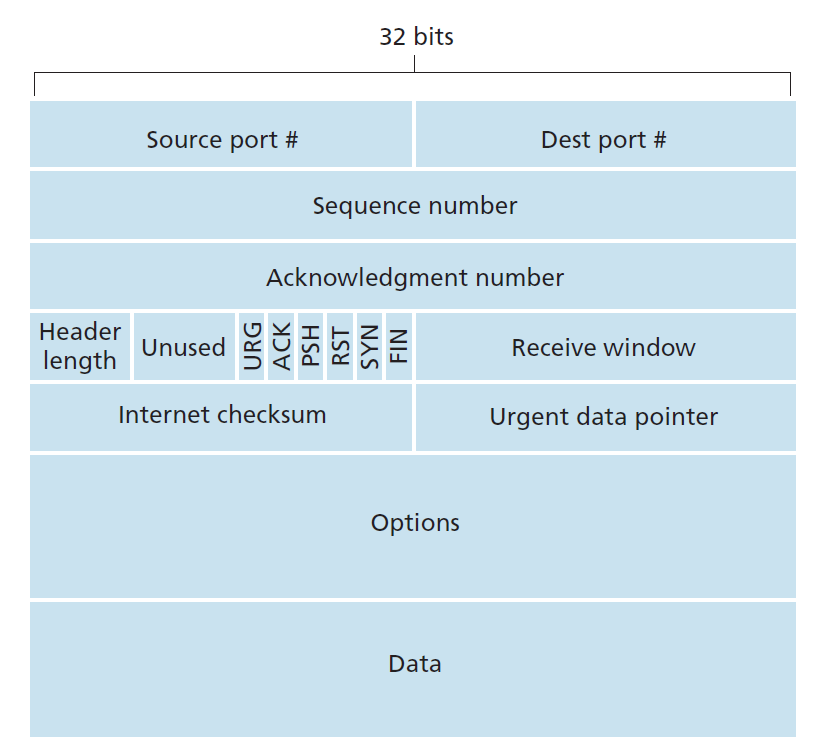
\includegraphics[width = 0.5\textwidth]{5_1_1.png}
\end{figure}
\subsubsection{Sequence Number}
\TCP sequence number refers to the "byte number" of the first byte of data transferred in the segment in the file. Note the sequence number is $0$-indexed.\\The first sequence number used in handshake is randomly selected and this randomly selected number will be used as offset for all subsequent sequence number.
\subsubsection{\TCP ACK Number}
\TCP Acknowledgement number records the sequence number of the \textit{next} byte of data \textit{expected} by receiver.\\

\TCP implements \textbf{cumulative} acknowledgement, in a sense \TCP ACKs up to the first missing byte in the stream.\\

However, \TCP spec doesn't say how receiver should handle out-of-order segments - it's up to implementer.\\

The $A$ bit in the header:
\begin{itemize}
  \item $A=0$ denotes a data packet
  \item $A=1$ denotes a ACK packet
\end{itemize}
There is only 1 timer running on the sender side.
\subsubsection{\TCP Sender Behaviour}
\begin{itemize}
  \item Event: \texttt{data} received from application above
  \begin{enumerate}
    \item Create \TCP segment with sequence number \texttt{NextSeqNum}
    \item Start timer if it is not running
    \item Send the packet
    \item Update sequence number used by next segment:\texttt{NextSeqNum = NextSeqNum + length(data)}
    \item Send until sender window is full.
  \end{enumerate}
  \item Event: Timer timeout
  \begin{enumerate}
    \item Retransmit not-yet-acknowledged segment with \textit{smallest} sequence number\footnote{Only the oldest unACKed packet is retransmitted}
    \item Start timer
  \end{enumerate}
  \item Event: ACK received, with ACK field value \texttt{y}
  \begin{enumerate}
    \item If \texttt{y>send\_base}, shift sender window: \texttt{send\_base=y}.
    \item If there are currently any not-yet-acknowledged segment, start timer.
  \end{enumerate}
\end{itemize}
\subsubsection{\TCP Receiver Behaviour}
\begin{itemize}
  \item Event: Arrival of in-order segment with sequence number \texttt{seqNum}
  \begin{itemize}
    \item if all data up to \texttt{seqNum} are already ACKed, wait up to 500ms for next segment. Send ACK if no next segment arrival.
    \item if one other segment is awaiting to send ACK, send single cumulative ACK, to ACK both in-order segment
    \end{itemize}
  \item Event: Arrival of out-of-order segment with higher than expected \texttt{seqNum}(gap formed and detected)
  \begin{itemize}
  \item Immediately send \textbf{duplicate} ACK, indicating \texttt{seqNum} of next expected segment\footnote{i.e. ACK the last correctly received packet}
  \end{itemize}
  \item Event: Arrival of segment that partially or completely fills gap
  \begin{itemize}
  \item Immediately send ACK, provided that the segment starts at lower end of gap.
  \end{itemize}
  \end{itemize} 
  \subsubsection{\TCP Timeout Value}
  \TCP computes and keeps updating timeout interval based on estimated RTT.
  \begin{align*}
  \text{Estimated RTT} &= (1-\alpha)\times\text{ Estimated RTT }+\alpha\times\text{ Sample RTT}\\
  &\text{typical value of }\alpha = 0.125\\
  \text{DevRTT} &= (1-\beta)\times\text{ DevRTT}+\beta\times|\text{SampleRTT --EstimatedRTT}|\\
  &\text{typical value of }\beta = 0.25\\
  \text{TimeoutInterval} &=\text{EstimatedRTT } +4\times\text{ DevRTT}
  \end{align*}
  \subsubsection{\TCP Fast Retransmission}
  \TCP adopts \textbf{fast retransmission} if sender receives 3 duplicate ACKs for the same data\footnote{1+3 = 4 ACKs of the same data in total}, it supposes that  segment after the last ACKed segment is lost. Thus it will resend segment before timer expires\footnote{Retransmission will not reset the timer}.
  \subsubsection{Establishing Connection}
  Before exchanging data, \TCP sender and receiver "shake hands".
  \begin{enumerate}
    \item Client chooses initial sequence number $x$, and send \TCP SYN msg, by setting $S= 1$.
    \item Server chooses initial sequence number $y$, and send \TCP SYNACK msg, by setting $A = 1$,$S=1$.
    \item Client sends ACK msg by setting $A=1$. In this message, it can contain client-to-server data.
  \end{enumerate}
  \subsubsection{Closing Connection}
  Client and server will close their side of connection by
  \begin{enumerate}
    \item Client sends FIN msg by setting $F=1$. After this segment sent, client can no longer send application data, but can receive data.
    \item Server send ACKFIN msg by setting $A = 1$, $F = 1$. Server can no longer send application data after this segment.
    \item Client sends ACK mssg by setting $A = 1$.
  \end{enumerate}
  \clearpage
\section{Network Layer}
Network layer is responsible for delivering packets to receiving hosts. Routers will examine header fields of \IP datagrams passing it and direct it to the right destination.
\subsection{\IP Address}

\begin{definition}[{\IP}v4 address]
\hfill\\\normalfont {\IP}v4 address is a 32-bit binary integer used to identify a host.
\end{definition}
A host can get an \IP address either
\begin{itemize}
  \item manually configured by system administrator, or
  \item automatically assigned by a DHCP server.
\end{itemize}
\subsection{Dynamic Host Configuration Protocol(DHCP)}
DHCP allows a host to dynamically obtain its \IP address from DHCP server when it joins network. It has the following benefits:
\begin{itemize}
  \item \IP address is renewable
  \item allow reuse of address (only hold address while connected)
  \item support mobile users who want to join network
\end{itemize}
\begin{theorem}[DHCP \IP assignment]\hfill\\\normalfont
Assignment of \IP address by DHCP server involves a 4-step process:
\begin{enumerate}
  \item Host broadcasts "DHCP \textbf{discover}" message\\
  \underline{Format}:\\
  \texttt{src: 0.0.0.0:68}\\
  \texttt{dest: 255.255.255.255:67}\\
  \texttt{yiaddr: 0.0.0.0}\\
  \texttt{transaction ID: 654}
  \item DHCP server responds with "DHCP \textbf{offer}" message\\
  \underline{Format}:\\
  \texttt{src: 223.1.2.5:67} (\IP address of DHCP server)\\
  \texttt{dest: 255.255.255.255:68}\\
  \texttt{yiaddr: 223.1.2.4}\\
  \texttt{transaction ID:654}\\
  \texttt{lifetime: 3600 secs}
  \item Host requests \IP address: "DHCP \textbf{request}" message\\
  \underline{Format}:\\
  \texttt{src: 0.0.0.0:68}\\
  \texttt{dest: 255.255.255.255:67}\\
  \texttt{yiaddr: 223.1.2.4}\\
  \texttt{transaction ID: 655}\\
  \texttt{lifetime: 3600 secs}
  \item DHCP server sends address: "DHCP \textbf{ACK}" message\\
  \underline{Format}:\\
  \texttt{src: 223.1.2.5:67}\\
  \texttt{dest: 255.255.255.255:68}\\
  \texttt{yiaddr: 223.1.2.4}\\
  \texttt{transaction ID: 655}\\
  \texttt{lifetime: 3600 secs}
\end{enumerate}
\end{theorem}
In addition to host \IP address assignment, DHCP may also provide a host additional network information, such as
\begin{itemize}
  \item \IP address of first-hop router
  \item \IP address of local DNS server
  \item Network Mask(network prefix)
\end{itemize}
Note, DHCP runs over \UDP 
\begin{itemize}
  \item DHCP server port number: 67
  \item DHCP client port number: 68
\end{itemize}
\subsection{Special \IP address}
\begin{table}[h]
\centering
\begin{tabular}{| p{3.4cm}|p{10cm}|}
\hline
Special Addresses&Present Use\\\hline
\begin{minipage}{3.3cm} \centering 0.0.0.0/8\end{minipage}&\textbf{Non-routable meta-address} for special use\\\hline
\begin{minipage}{3.3cm} \centering 127.0.0.0/8\end{minipage}& \begin{minipage}{9.9cm}\textbf{Loopback address}\\ A datagram sent to an address within this block loops back inside the host. \\This is ordinarily implemented using only 127.0.0.1/32.\end{minipage}\\\hline
\begin{minipage}{3.3cm}\centering 10.0.0.0/8\\172.16.0.0/12\\192.168.0.0/16\end{minipage}&\begin{minipage}{9.9cm}\textbf{Private addresses}\\They can be used without any coordination with IANA or an Internet registry.\end{minipage}\\\hline
\begin{minipage}{3.3cm}\centering 255.255.255.255/32\end{minipage}&\begin{minipage}{9.9cm}\textbf{Broadcast address}\\All hosts on the same subnet receive a datagram with such a destination address.\end{minipage}\\\hline
\end{tabular}
\end{table}
\subsection{\IP address and Network Interface}
An \IP address is associated with a \textbf{network interface}.
\begin{itemize}
  \item A host usually has one or two network interfaces(e.g. wired Ethernet and WiFi).
  \item A router typically has multiple interfaces (e.g. subnet)
\end{itemize}
\subsubsection{\IP address and Subnet}
An \IP address logically comprises two parts:
\[
\overbrace{\underbrace{\text{Network (subnet) prefix}}_{n \text{ bits}}|\underbrace{\text{host ID}}_{32-n \text{ bits}}}^{32 \text{bits}}
\]
\begin{definition}[Subnet]\hfill\\\normalfont
\textbf{Subnet} is a network formed by a group of "directly" interconnected hosts.
\end{definition}
\begin{theorem}[Properties of subsets]
\hfill\\\normalfont
\begin{itemize}
  \item Hosts in the same subnet have the \textit{same} network prefix in their \IP address.
  \item Hosts in the same subnet can physically reach each other \textit{without} intervening router.
  \item They connect to the outside world through a router.
  \end{itemize}
\end{theorem}
\subsection{\IP address assignment in Internet}
Internet's \IP address assignment strategy is known as \textbf{Classless Inter-domain Routing}(CIDR). For corporations, they will be offered with a continuum of \IP address with fixed subnet prefix by an ISP.
\begin{itemize}
  \item Subnet prefix of \IP address is of arbitrary length.
  \item Address format: \texttt{a.b.c.d/x}, where \texttt{x} is the number of bits in subnet prefix of \IP address.
\end{itemize}
\textbf{Subnet mask} is used to determine which subnet an \IP address beong to.\\Subnet mask is calculated by setting all subnet prefix bits to 1 and hosts ID bits to 0.
\subsection{Hierarchical Addressing}
This hierarchical addressing via restricting subnet prefix at all levels allows efficient advertisement of routing information. \\Router uses \textbf{longest prefix match} in forwarding table when determining to which next hop a \IP datagram is sent.
\clearpage
\section{\IP{ and Routing}}
\subsection{\IP{v4} Datagram Format}
\begin{figure}[h]
\centering
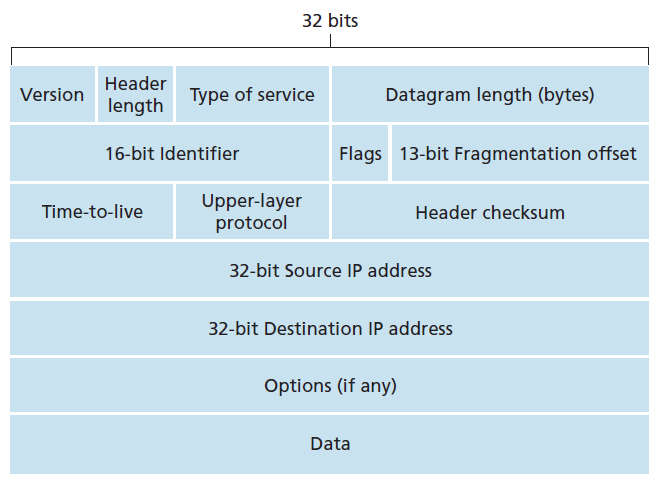
\includegraphics[width = 0.7\textwidth]{6_1_1.png}
\end{figure}
The key fields in the \IP{v4} datagram are the following
\begin{itemize}
  \item Version Number: These 4 bits specify the \IP protocol version.
  \item Datagram length: Total length of \IP datagram (header \textit{plus} data), measured in \textbf{bytes}.
  \item Identifier, flags, fragmentation offset are used in \IP fragmentation.
  \item Time-to-live(TTL) refers to number of remaining hops, decremented at each router
  \item Header checksum is used to detect error for the \IP header
  \item source and destination \IP address refers to the initial sender and final receiver's \IP address
\end{itemize}
A typical \IP{v4} header is 20 bytes long.
\subsection{\IP Fragmentation and Reassembly}
\IP fragmentation is used as different links may have different \textbf{maximum transfer unit}(MTU) specified by underlying link layer, and \IP datagrams could be so large that need to be fragmented to fit into MTU.
\begin{figure}[h]
\centering
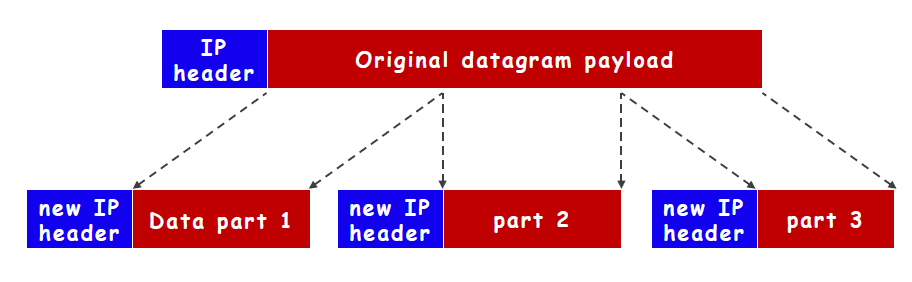
\includegraphics[width = 0.6\textwidth]{6_2_1.png}
\end{figure}
When destination hosts reassembles the packet, \IP header fields are used to identify fragments and their relative order.
\textbf{Flag}: flag is set to 
\begin{itemize}
  \item 1 if there is next fragment from the same segment
  \item 0 if this is the last fragment
\end{itemize}
\textbf{Offset}: offset is expressed in unit of 8-bytes, indicating the first byte of the data of this datagram in relative to the original fragmented datagram.\\
\textbf{ID}: Same datagram will use the same ID.\\
\textbf{Length}: Length field will change accordingly in smaller packets.
\subsection{Intra-AS Routing}
The Internet is a network-of-networks, organised in a hierarchy of \textbf{autonomous systems}(AS). \\Due to the size of the Internet and the decentralised administration of the Internet, routing on the Internet is done \textbf{hierarchically}:
\begin{itemize}
  \item Intra-AS routing
  \begin{itemize}
    \item Finds a good paths between two routers within an AS.
    \item Commonly used protocols: RIP, OSPF
  \end{itemize}
  \item Inter-AS routing
  \begin{itemize}
    \item Handles the interfaces between ASes.
    \item The de facto standard protocol: BGP
  \end{itemize}
\end{itemize}
\begin{figure}[h]
\centering
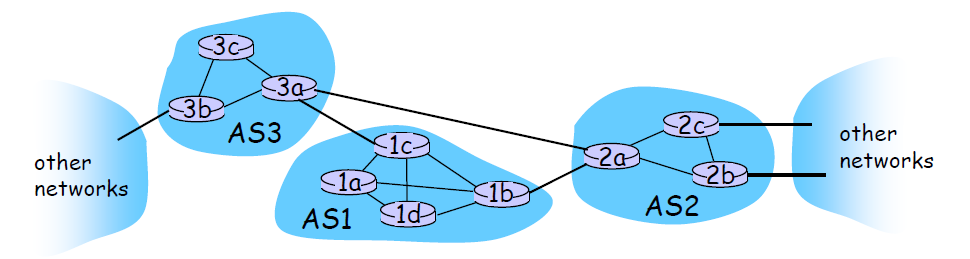
\includegraphics[width = 0.7\textwidth]{7_2_1.png}
\end{figure}
The aim of routing may differ between intra-AS routing and inter-AS routing.
\begin{itemize}
  \item Intra-AS routing
  \begin{itemize}
    \item Single admininistrator, so no policy decisions in needed.
    \item Routing mostly focus on performance.
  \end{itemize}
  \item Inter-AS routing
  \begin{itemize}
    \item Administrator often wants to control over how its traffic is routed, who routes through its net, etc.
    \item Policy may dominate over performance
  \end{itemize}
\end{itemize}
We can abstractly view a network of routers as a \textit{graph}, where vertices are routers and edges are physical links between routers.\\
Costs can be associated to each link, represented as the weight of respective edge. 

In this sense, routing is the problem of finding a least cost path between two vertices in a graph.
\subsubsection{Link State Algorithm}
For link state algorithm, \textit{all} routers have the complete knowledge of network topology and link cost. Routers will periodically broadcast link costs to each other.

The least cost path can be found using dijkstra algorithm.
\subsubsection{Distance Vector Algorithm}
Routers know \textit{physically-connected neighbours} and \textit{link costs to neighbours}. Router exchange \textbf{local views} with neighbours and update own local view, based on neighbours' view.

It admits an iterative process of computation converging slowly:
\begin{itemize}
  \item Swap local view with \textit{direct} neighbours.
  \item Update own's local view.
  \item Repeat 1 -- 2 till no more change to local view.
\end{itemize}
Let $c(x,y)$ be the cost of link between routers $x$ and $y$. $c(x,y) = \infty$ if $x$ and $y$ are note direct neighbours. \\Let $d_x(y)$ be the cost of the \textit{least}-cost path from $x$ to $y$, from $x$ point of view. This $d$ is called teh distance vector.

Distance vector algorithm then utilises Bellman-Ford Equation:
\[
d_x(y) = \min_{v\text{ neighbour of }x}\{c(x,v)+d_v(y)\}
\]
The first term is easily obtained since it is mostly manually configured. The distance vector in second term is obtained from exchange of local views between neighbours.
\subsubsection{Bellman-Ford behaviour}
Router will maintain a $N\times N$ table where $N$ is number of routers in the network, storing $d_\text{from}(\text{to})$.
\begin{itemize}
\item In the beginning, router $x$ has only $c(x,v)$ known. $c(x,v)$ is $\infty$ if $v$ is not a neighbour. Therefore, $d_x(v)$ is initialised as $c(x,v)$ and others to infinity.
\item Router will exchange $d_\cdot(v)$ with each other. After each exchange, $x$ will update $d_x(v)$ according to Bellman-Ford Equation.
\item In addition, $x$ will note down the next hop router to every destination, based on the least cost path. This information will be used to create forwarding table of $x$.
\item Eventually this table will converge to provide optimal routing service.
\end{itemize}
\subsection{Routing Information Protocol(RIP)}
\begin{itemize}
\item Routing Information Protocol implements the Distance Vector Algorithm. It uses \textbf{hop counts} as the cost metric.\footnote{Therefore, it has the drawback of being insensitive to network congestion.}\\
\item Entries in the routing table are aggregated subnet masks.
\item Routers exchange routing table every 30 seconds over \UDP port 520.
\item Self-repair mechanism: if there is no update from a neighbour router for 3 minutes, the neighbour is assumed to be failed.
\end{itemize}
\subsection{Network Address Translation(NAT)}
Network Address Translation is used by routers connecting to both local network and the internet, for translating \IP addresses with the aid of port number. \\It is necessary since private \IP addresses cannot be used for routing on the Internet.
\subsubsection{Implementation of NAT}
NAT enabled routers must:
\begin{itemize}
  \item Maintain a NAT translation table, in which mapping between (source \IP address, port \#) of the private network and (NAT \IP address, \textit{new} port \#) used on the Internet are stored.
  \item For \textbf{outgoing} datagrams, replace (source \IP address, port \#) to (NAT \IP address, \textit{new} port \#).
  \item For \textbf{incoming} datagrams, replace (NAT \IP address, \textit{new} port \#) in destination fields with coresponding (source \IP address, port \#) by NAT translation table.
\end{itemize} 
The benefits of NAT include:
\begin{itemize}
  \item There is no need to rent a range of public \IP addresses from ISP, just one public \IP for the NAT router.
  \item All hosts use private \IP addresses. Addresses of hosts in local network without notifying the outside world.
  \item ISP can be changed without changing addresses of hosts in local network.
  \item Hosts inside local network are not explicitly addressable and visible by outside world.
\end{itemize}
\subsection{Internet Control Message Protocol(ICMP)}
Internet Control Message Protocol(ICMP) is used by hosts and routers to communicate network-level information.
\begin{itemize}
  \item Error reporting: unreachable host / netowrk / port / protocol
  \item Echo request/reply (used by \texttt{ping})
\end{itemize}
ICMP messages are carried in \IP datagrams. ICMP header starts \textbf{after} \IP header.
\begin{table}[h]
\centering
\begin{tabular}{|c|c|c|}\hline
Type&Code&Description\\\hline
8&0&echo request(\texttt{ping})\\\hline
0&0&echo reply(\texttt{ping})\\\hline
3&1&dest host unreachable\\\hline
3&3&dest port unreachable\\\hline
11&0&TTL expired\\\hline
12&0&bad \IP header\\\hline
\end{tabular}
\end{table}
\subsubsection{\texttt{ping} and \texttt{traceroute}}
Command \texttt{ping} sees if a remote host will respond to us -- check for connection.

Command \texttt{traceroute} sends a series of small packets across a network and attempts to display the route (or path) that the messages would take to get to a remote host.
\clearpage
\section{Network Security}
Network security concerns about the following aspects:
\begin{itemize}
\item Message confidentiality
\item Message integrity
\item Message authenticity
\item Service availability
\end{itemize}
Let us denote the two parties of communication as Alice and Bob, and the intruder as Trudy.
\subsection{Principles of Cryptography}
Cryptography is aimed to make it difficult for an unauthorised third party to understand private communications.\\
Cryptography involves both \textbf{algorithms}, which is known public, and \textbf{keys}, which are dependent on the type of algorithms used, and is kept secret.\\
Suppose Alice has an encryption key $K_A$ and Bob has a corresponding decryption key $K_B$, the following relationship is preserved
\[
K_B(K_A(m))=m
\]
where $m$ is the message Alice wants to send to Bob.\\
There are two types of cryptography, namely \textbf{symmetric key} cryptography and \textbf{public key} cryptography.
\subsubsection{Symmetric Key Cryptography}
In symmetric key cryptography, Alice and Bob share and use the \textbf{same}(\textbf{symmetric}) key: $K_{A-B}$.\\Popular algorithms include Advanced Encryption Standard(AES).\\
One simplistic example of symmetric key cryptography is \textbf{monoalphabetic cipher}. In this scheme, Alice and Bob share an identical mapping table from a permutation of 26 letters to another permutation, for translation between plaintext and ciphertext.\\
Symmetric key cryptography has the following problem: sender and receiver cannot agree on the shared key in the first place.
\subsubsection{Public Key Cryptography}
In public key cryptography, each party has a pair of keys, namely the \textbf{public key}, $K^+$, and \textbf{private key}, $K^-$. The public key is known public and the private key is kept confidental. The choice of this pair of key requires:
\begin{enumerate}
  \item $K^-(K^+(m))=m$
  \item Given public key $K^+$, it should be very difficult to find private key $K^-$.
\end{enumerate}
The most popular algorithm of public key cryptography is \textbf{RSA}, for which, the public key is the product of two \textit{very large prime} numbers and the private key is derived from these two large primes.
\begin{theorem}[Property of RSA]
\hfill\\\normalfont An important property of RSA is that the public key and private key are commutative:
\[
K^-K^+=K^+K^-=1
\]
where $1$ is the identity operator.
\end{theorem}
RSA, although resolves the problem of key sharing, is \textit{computationally intensive}, thus slower. Therefore in practive, the following standard is used:
\begin{enumerate}
  \item Use public key cryptography to establish secure connection, by exchanging the symmetric session key $K_S$.
  \item Then use this session key for encryption and decryption.
\end{enumerate}
Note that $K_S$ is only valid for \textit{one} session.
\subsection{Message Integrity and Digital Signatures}
Two ways to ensure message integrity and meesage authenticity are \textbf{message authentication code}(MAC) and \textbf{digital signature}.
\subsubsection{Cryptographic Hash Function}
Cryptographic hash function is the basis of both methods above.
\begin{definition}[Cryptographic Hash Function]
\hfill\\\normalfont Cryptographic hash function is a hash function $H$ which takes an input $m$, and generate a \textit{fixed size} string $H(m)$, known as \textbf{message digest}(hash or finger print).\\
Cryptographic hash function must adhere the property that it is computationally infeasible to find two different messages $m$ and $m^\prime$ such that $H(m)=H(m^\prime)$.
\end{definition}
The following property makes it impossible for Trudy to forge another message $m^\prime$ with the same message digest as $m$.\\
Popular cryptographic hash functions include MD5 and SHA-1.
\begin{theorem}[Work Flow of hash function]
\hfill\\\normalfont For Alice, the sender of the message.
\begin{enumerate}
  \item Alice creates message $m$ and calculates the hash $H(m)$.
  \item Alice then appends $H(m)$ to the message $m$, creating an extended message $(m, H(m))$, and sends the extended message to Bob.
\end{enumerate}
For Bob, the receiver,
\begin{enumerate}
  \item Bob receives an extended message $(m^\prime, h^\prime)$.
  \item Bob calculates $H(m^\prime)$. If $H(m^\prime)=h^\prime$, Bob concludes that message integrity is preserved.
\end{enumerate}
\end{theorem}
However, cryptographic hash function does not guarantee message authenticity, which leads to the invention of message authentication code.
\subsubsection{Message Authentication Code}
To ensure message authenticity, Alice and Bob agrees on a \textbf{message authentication code}, $s$. The extended work flow is as follows:
\begin{theorem}[Work Flow of message authentication code]
\hfill\\\normalfont For Alice, the sender of the message.
\begin{enumerate}
  \item Append, by method of string concatenation, $s$ after $m$ to form the modified message $m+s$.
  \item Calculate the hash $H(m+s)$.
  \item Alice then appends $H(m+s)$ to the message $m$, creating an extended message $(m, H(m+s))$, and sends the extended message to Bob.
\end{enumerate}
For Bob, the receiver,
\begin{enumerate}
  \item Bob receives an extended message $(m^\prime, h^\prime)$.
  \item Bob calculates $H(m^\prime+s)$. If $H(m^\prime+s)=h^\prime$, Bob concludes that message integrity \textbf{and} message authenticity are preserved.
\end{enumerate}
\end{theorem}
\subsubsection{Digital Signature}
The problem of message authentication code is that either Bob and Alice could produce the same $H(m+s)$. Therefore, the producer of the message cannot be uniquely identified.\\
Digital signature, which solves this problem, has the following properties:
\begin{itemize}
  \item \textbf{verifiable}: recipient(Bob) can verify that Alice, and \textbf{no one else}, has signed the document.
  \item \textbf{non-repudiation}: when presented the document and digital signature to a third party, the third party is confident that this document is indeed signed by Alice but no one else.
\end{itemize}
One way to produce the digital signature is to utilise the \textbf{private key} of the public key encryption scheme.
\begin{theorem}[Work flow of Digital Signature]
\hfill\\\normalfont 
For Alice,
\begin{itemize}
\item Alice signs $m$ be encrypting the message digest $H(m)$ with her private key $K_A^-$, creating a ``signed'' message digest $K_A^-(H(m))$.
\item Alice sends both $m$ and $K_A^-(H(m))$ to Bob.
\end{itemize}
For Bob, he receives $(m^\prime, \text{signature})$
\begin{itemize}
  \item Verify the sender by computing the message digest $H(m)$.
  \item and compare with $K^+(\text{signature})$.
\end{itemize}
\end{theorem}
One problem of the above workflow is that, the public key Bob uses may not definitely be Alice's. To resolve this issue, certificate authority is used.\\\textbf{Certificate authority} is an entity that issues digital certificates, which is Alice's public key encrypted by Certificate Authority's private key, i.e. $K_\text{CA}^-K_A^+$.\\If Bob trusts the certificate authority's public key, it will trust Alice's public key, by applying $K_\text{CA}^+(DC)$.
\subsection{Security Layer}
\subsection{SSL: Secure Socket Layer}
Secure socket layer is an layer interfaced between application and transport layer. It is applicable to \TCP conenctions.
\subsection{IPSec: Internet Protocol Security}
IPsec is a suite of protocols that secure communications by authenticating and ecrypting each \IP packet of a communication session. It is interfaced between Transport layer and \IP layer.\\Both SSL and IPsec can be used to build VPN. 
\clearpage
\section{Link Layer}
\textbf{Link Layer} is responsible of sending datagrams between adjacent nodes over a \textit{single} link.
\begin{itemize}
  \item \IP datagrams are encapsulated in link-layer \textbf{frames} for transmission.
  \item Different link-layer protocols may be used on different links;\\each protocol may provide a different set of services.
\end{itemize} 
Link layer may offer the following services
\begin{itemize}
  \item \textbf{Framing}: encapsulate \IP datagram into link-layer fram, adding header and trailer\\\textbf{Remark}: different protocols have different header and trailer format; each header and trailer is valid for \textit{only one} hop
  \item \textbf{Link access control}: Coordinate which nodes can send frames at a certain point of time, when multiple nodes \textit{share} a single link.
  \item \textbf{Reliable delivery}
  \item \textbf{Error detection}
  \begin{itemize}
    \item Errors are usually caused by signal attenuation or noise.
    \item Receiver detedcts presence of errors. Receiver, when error is detected, may signal sender for retransmission or simply drop frame.
  \end{itemize}
  \item \textbf{Error correction}: Receiver may identify and correct bit error without resorting to retransmission.
\end{itemize}
Link layer is implemented in adapters, which contain both link and physical layer.
\subsection{Error Detection and Correction}
Commonly used error detection schemes include
\begin{itemize}
  \item Checksum(used in \TCP/\UDP/\IP)
  \item Parity Checking
  \item CRC(commonly used in link layer)
\end{itemize}
Note that error detection schemes are not 100\% reliable.
\subsubsection{Parity Checking}
\begin{definition}[Single Bit Parity]
\hfill\\\normalfont Suppose the data is of the form of $d_n\cdots d_1$, the parity bit $p$ is chosen such that
\[
\sum_{i=1}^n d_i + p \equiv 0 \;\;\;\mod 2
\]
The sender, after computing the parity, will send data and parity bit, in the form of $d_n\cdots d_1 p$.
\end{definition}
\begin{definition}[Two-dimensional Bit Parity]
\hfill\\\normalfont In two-dimensional bit parity, the data is arranged in a two-dimensional array, and the single bit parity is computed for each row and column. The augmented array with both data and parity bits will be sent.\\Two-dimensional bit parity can
\begin{itemize}
  \item Detect \textbf{and correct} single bit errors in data.
  \item Detect two bits errors in data.
\end{itemize} 
\end{definition}
\subsubsection{Cyclic Redundancy Check(CRC)}
Cyclic Redundancy check is a power error-detection coding. It consists of
\begin{itemize}
  \item $D$: data bits viewed as a binary number
  \item $G$: generator of length $(r+1)$ bits, agreed by sender and receiver beforehand
  \item $R$: CRC checksum in length of $r$ bits
\end{itemize}
CRC checksum is computed as follows:
\begin{enumerate}
  \item Append $r$ bits of 0's after the data $D$.
  \item Perform bitwise \texttt{XOR} operation on the augmented data $D\underbrace{0\cdots 0}_{r\text{ bits}}$.\\This \texttt{XOR} operation is done withour carry or borrow, between augmented data and $G$. The operations starts from the MSBs of augmented data and cascading to the LSBs.
  \item The remainder will be set as $R$, which replaces the trailing 0's in augmented data, to form the CRC checksum $D+R$, where $+$ is the string contacenation.
\end{enumerate}
If $G\nmid D+R$, the error is detected. 
\subsection{Multiple Access Links and Protocols}
There are two types of network links, namely
\begin{enumerate}
  \item \textbf{Point-to-point link}, where a sender and receiver connected by a \textbf{dedicated} link, which do not need multiple access contol
  \item \textbf{Broadcast link}, where
  \begin{itemize}
    \item Multiple nodes connected to a shared broadcast channel
    \item When a node transmits a frame, the channel broadcasts the frame and each other node receives a copy
  \end{itemize}
\end{enumerate}
In a broadcast channel, if two or more nodes transmit simultaneously, frames will \textbf{collide} at nodes and \textbf{none} will be correctly read.\\
Therefore, multiple access protocol is required, to serve as an distributed algorithms that determines how the nodes share the channel, using the channel itself.\\
Multiple access protocols can be categorised into three broad classes:
\begin{enumerate}
  \item \textbf{Channel Partitioning}: divide channel into smaller "pieces"; pieces are allocated to nodes for \textbf{exclusive} use.
  \item \textbf{Taking turns}: nodes take turns to transmit
  \item \textbf{Random access}: channel are not divided so collisions are still possible; the mechanism focuses on recovery from collision.
\end{enumerate}
\subsubsection{Channel Partitioning Protocols}
\begin{definition}[Time Division Multiple Access(TDMA)]
\hfill\\\normalfont 
\begin{itemize}
\item The channel is divided into equal time slots.
\item Access to channel will be in ``rounds'', where each node gets \textbf{fixed} length slots(equivalently, equal transmission time) in each round.
\item Unused slots go idle.
\end{itemize}
\end{definition}
\begin{definition}[Frequency Division Multiple Access(FDMA)]
\hfill\\\normalfont 
\begin{itemize}
\item Channel spectrum is divided into frequency bands.
\item Each node is assigned a \textbf{fixed} frequency band.
\item Unused transmission frequency bands go idle.
\end{itemize}
\end{definition}
\subsubsection{``Taking Turns'' Protocols}
\begin{definition}[Polling]
\hfill\\\normalfont
\begin{itemize}
\item In polling, there is a \textbf{master} and rest of the nodes are the \textbf{slaves}.
\item Master nodes invites slave nodes to transmit in turn.
\end{itemize}
\end{definition}
Concerns of polling include (1)polling overhead and (2)single point of failure (at master node).
\begin{definition}[Token Passing]
\hfill\\\normalfont \begin{itemize}
\item In token passing, there is a \textbf{control token}. 
\item Control token is passed from one node to next sequentially.
\item Only the node with the control token can send. \end{itemize}
\end{definition}
Concern of token passing include (1)token overhead and (2)single point of failure (at control token).
\subsubsection{Random Access Protocols}
For random access protocols, when node has packet to send, there is no \textit{a priori} coordination among nodes. A consequence is the presence of \textbf{collision}.\\Random access protocols instead specify:
\begin{itemize}
  \item How to detect collisions
  \item How to recover from collisions
\end{itemize}
\begin{definition}[Slotted ALOHA]
\hfill\\\normalfont In slotted ALOHA,
\begin{itemize}
  \item All frames require to have equal size.
  \item Time is divided into slotes of equal length.
  \item Node start to transmit only at the beginning of a slot.
\end{itemize}
The operation of each node includes
\begin{itemize}
\item \textbf{Collision Detection}: listens to the channel while transmissing
\item \textbf{Collision resolution}: if collision happens, node retransmits a frame in \textit{each subsequent} slot with probability $p$ until success/
\end{itemize}
\end{definition}
\begin{definition}[Pure ALOHA]
\hfill\\\normalfont In pure ALOHA, there is no requirement of slot nor synchronisation: when there is a fresh frame, transmit immediately.\\Therefore, the chance of collision increases.
\end{definition}
In fact, collision is the main issue of efficiency. 
\begin{definition}[Carrier Sense Multiple Access(CSMA)]
\hfill\\\normalfont CSMA senses the channel before transmission and 
\begin{itemize}
  \item if channel is \textit{sensed idle}, transmit frame
  \item if channel is \textit{sensed  busy}, defer transmission
\end{itemize}
\end{definition}
\textbf{Remark}:\\ Collision may still happen in CSMA. One scenario is when two nodes sense the channel idle at the same time and both start transmission.\\
Even different nodes sense channel at \textit{different} time, collisions can still occur due to \textbf{propagation delay}.

One issue of CSMA is that node may not detect collision if the frame size is too small. Therefore, a \textbf{minimum frame size} is imposed on the frame. Payload will be padded with 0 at the back if necessary to achieve minimum frame size.\\For example, Ethernet requires a minimum of frame size of 64 bytes.
\begin{definition}[CSMA/CD]
\hfill\\\normalfont CSMA/CD (Collision Detection) is an extension from CSMA. It specifies the following rules:
\begin{itemize}
  \item When collision is detected, transmission is aborted, to reduce channel wastage.
  \item Retransmit after a random amount of time.
\end{itemize}
\end{definition}
\begin{definition}[CSMA/CA]
\hfill\\\normalfont CSMA/CA (Collision Avoidance) is an extension from CSMA. It specifies the receiver to return ACK if a frame is received OK and NAK if not.
\end{definition}
CSMA/CA is used in 802.11 as collision detection by hosts is difficult in wireless context.
\clearpage
\section{Local Area Network}
\subsection{Link Layer Addressing \& ARP}
\subsubsection{MAC address}
\begin{definition}[MAC address]
\hfill\\\normalfont Every adaptor has a \textbf{MAC address} aka physical or LAN address. MAC address is used to send and receive link layer frames.\\
MAC address is typically 48 bits long, the first three bytes of which identifies the vendor of an adaptor.
\end{definition}
Adapter handles frames by checking if the destination MAC address of the frame matches its own MAC address.
\begin{itemize}
  \item If yes, adapter extracts the enclosed datagram and passes it to the protocol stack.
  \item If no, adaptor discards the frame without interrupting the host.
\end{itemize}
The key difference between \IP address and MAC address is that, \IP address is dynamically assigned and hierarchical to facilitate routing, whereas MAC address is permanent for the identification of the hardware.
\subsubsection{Address Resolution Protocol(ARP)}
Address Resolution Protocol is used to translate the \IP address to the MAC address.\\Each \IP node has an ARP table, in which mappings of \IP address and MAC address of other nodes in the \textbf{same subnet} is stored, in the following format:
\[
\langle\IP \text{ address, MAC address, TTL}\rangle
\]
\begin{theorem}[Workflow of ARP in Subset]
\hfill\\\normalfont Suppose node $A$ sends frames to node $B$ in the same subnet,
\begin{itemize}
  \item If node $A$ has MAC address of node $B$ in its ARP table, node $A$
  \begin{itemize}
    \item creates a frame with $B$'s MAC address and send it.
    \item Only node $B$ will process this frame.
    \item All other nodes will receive but ignore this frame/
  \end{itemize} 
  \item If node $A$ do not have MAC address of node $B$ in the ARP table, node $A$
  \begin{itemize}
    \item \textbf{broadcast} an ARP query packet, containing $B$'s \IP address
    \begin{itemize}
      \item Destination MAC address set to FF-FF-FF-FF-FF-FF
      \item All nodes in the same subnet will receive this ARP query packet, but only node $B$ will \textbf{reply} it.
    \end{itemize}
    \item node $B$ replies to node $A$ with its MAC address.
    \item node $A$ caches $B$'s \IP-to-MAC address mapping in its ARP table.
    \item node $A$ then follows the steps of the first bullet point.
  \end{itemize}
\end{itemize}
\end{theorem}
\begin{theorem}[Workflow of ARP between Subset]
\hfill\\\normalfont If node $B$ is not in the same subset as node $A$, node $A$, when transmitting frames, should create a link layer frame with
\begin{itemize}
  \item $R$'s MAC address as destination MAC address, where $R$ is the router interfaced with $A$
  \item $B$'s \IP address as destination \IP address.
\end{itemize}
When the packet reaches the router $R$, $R$ will move datagram to outgoing link by constructing a new frame with $B$'s MAC address.
\end{theorem}
\subsection{Ethernet}
\begin{definition}[Local Area Network]
\hfill\\\normalfont Local Area Network(LAN) is a computer network that interconnects computers within a geographical area such as office building or university campus.
\end{definition}
LAN technologies include:
\begin{itemize}
  \item IBM Token Ring
  \item Ethernet
  \item Wi-Fi
  \item Others
\end{itemize}
\textbf{Ethernet} is the dominant \textit{wired} LAN technology. It comprises of a series of Ethernet standards of different speeds, different physical layer media, but \textbf{MAC protocol} and \textbf{frame format} remain unchanged.

Ethernet has two physical topology, namely 
\begin{itemize}
\item \textbf{bus} topology, where all nodes can collide with each other
\item \textbf{star} topology, where the \textbf{switch} in center eliminates collision
\end{itemize}
\subsubsection{Ethernet Frame Structure}
Ethernet frame are of the following format:
\begin{figure}[h]
\centering
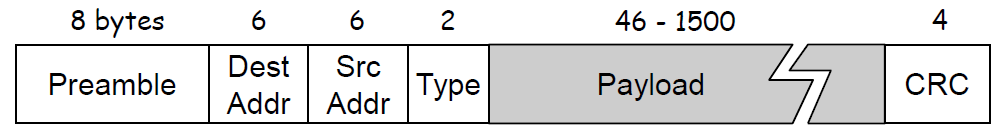
\includegraphics[width = 0.5\textwidth]{9_1_1.png}
\end{figure}
\clearpage
\textbf{Remark}: Preamble is not part of the Ethernet frame. It is
\begin{itemize}
  \item 7 bytes with pattern 10101010 followed by 1 byte with pattern 10101011
  \item used to synchronize receiver and sender clock rates.
\end{itemize}
The Ethernet frame has the following components:
\begin{itemize}
  \item \textbf{Source and Destination MAC address}
  \begin{itemize}
    \item If nodes receive a frame with matching destination address, or with \textbf{broadcast address}, it passes data in the frame to network layer protocol
    \item Otherwise, the frame is discarded
  \end{itemize}
  \item \textbf{Type}: indicates higher layer protocol
  \item \textbf{CRC}: used for error detection; corrupted frame will be dropped
\end{itemize}
\subsubsection{Ethernet Data Delivery Service}
Ethernet is
\begin{itemize}
  \item \textbf{Connectionless}: no handshaking required between sending and receiving nodes
  \item \textbf{Unreliable}: receiving nodes doesn't send ACK or NAK to sending nodes\\
  A consequence is that data in dropped frames will be recovered only if initial sender uses higher layer Reliable Data Trasfer Protocol.
  \item \textbf{Ethernet's multiple access protocol}: CSMA/CD with binary backoff
\end{itemize}
\begin{theorem}[Ethernet CSMA/CD Algorithm]
\hfill\\\normalfont
\begin{enumerate}
  \item Sending nodes receives datagram from network layer, and creates frame
  \item If channel is sensed idle, start frame transmission.\\If channel is sensed busy, waits until channel is sensed idle, then transmits
  \item If the entire frame is trasmitted without detecting another transmission, the frame is finished.
  \item If there is another transmission while transmitting, aborts and sends jam signal.
  \item After aborting, the nodes enters binary back-off:
  \begin{itemize}
    \item After $m$th collision, node chooses $K$ at random from $\{0,1,2,\ldots, 2^m-1\}$
    \item node waits $512K$ bit times and return to step 2.
  \end{itemize}
\end{enumerate}
\end{theorem}
\textbf{Remark}: sometimes there is an upper bound of $m$, after which the frame is dropped.
\subsection{Link Layer Switches}
\begin{definition}[Ethernet Switch]
\hfill\\\normalfont Ethernet switch is a link-layer device used in LAn that 
\begin{itemize}
  \item Store and forward Ethernet frames
  \item Examine incoming frames' MAC addresses and selectively forward frame to one-or-more outgoing links
\end{itemize}
\end{definition}
Ethernet switch has the following properties:
\begin{itemize}
\item Ethernet switch is transparent to hosts in the sense that it has no \IP address and hosts are unware of the presence of switches.
\item In Ethernet of star topology, hosts have dedicated connection to switch.
\item Switch buffers frames and is full duplex.
\item CSMA/CD is used on each link, despite no collisions.
\end{itemize}
\begin{definition}[Switch Forwarding Table]
\hfill\\\normalfont Each switch has a \textbf{switch table}, which stores entry of the following format:
\[
\langle\text{MAC address of host, interface to reach host, TTL}\rangle
\]
\end{definition}
\begin{theorem}[Self-learning of switch table]
\hfill\\\normalfont Switch learns which hosts can be reached through which interfaces. Specifically,
\begin{itemize}
  \item When receiving a frame from $A$, the location and interface of $A$ is noted down in switch table.
  \item If destination $B$ is found in the table, forward the frame onto that link.
  \item If destination $B$ is unknown, broadcast the frame to all outgoing links
  \item The destination $B$ will send the ACK signal, from which the switch learns the location and interface of $B$ and notes down them in the switch table.
\end{itemize}
\end{theorem}
\textbf{Remark}: Switches can be connected in hierarchy.
\end{document}